\documentclass[avery5371,grid]{flashcards}

\cardfrontstyle[\large\slshape]{headings}
\cardbackstyle{empty}


\usepackage{amssymb}
\usepackage{amsfonts}
\usepackage{amsmath} %allows me to use /begin{align*} and \dfrac{}{}
\usepackage{txfonts}
\usepackage{enumerate}
\usepackage{enumitem}
\usepackage{tikz}

\usetikzlibrary{decorations.markings}
\usetikzlibrary{arrows,shapes,positioning}

\newcommand{\R}{\mathbb{R}}
\newcommand{\N}{\mathbb{N}}
\newcommand{\Z}{\mathbb{Z}}
\newcommand{\C}{\mathbb{C}}
\newcommand{\Q}{\mathbb{Q}}
\newcommand{\F}{\mathbb{F}}
\newcommand{\K}{\mathbb{K}}
\newcommand{\vbar}{\; | \;}
\newcommand{\divides}{\bigm|}
\newcommand{\inv}{^{-1}}
\newcommand{\finlist}[2]{{#1}_1, {#1}_2, \ldots, {#1}_{#2}}
\newcommand{\inflist}[1]{{#1}_1, {#1}_2, {#1}_3, \ldots}
\newcommand{\paren}[1]{\left( #1 \right) }
\newcommand{\setbrace}[1]{\left \{ #1 \right \} }
\newcommand{\sqbrack}[1]{\left[ #1 \right] }
\newcommand{\rmod}{$R$-module}
\newcommand{\blank}{$\; \underline{\hspace{1in}} \; $}
% \renewcommand{\sum}{\sum \limits} % This keeps giving me an error!

\DeclareMathOperator{\Orb}{Orb}
\DeclareMathOperator{\Stab}{Stab}
\DeclareMathOperator{\Hom}{Hom}
\DeclareMathOperator{\Tor}{Tor}
\DeclareMathOperator{\img}{im}
\DeclareMathOperator{\End}{End}
\DeclareMathOperator{\Ann}{Ann}
\DeclareMathOperator{\vspan}{span}
\DeclareMathOperator{\sgn}{sgn}
\DeclareMathOperator{\tr}{trace}
\DeclareMathOperator{\rank}{rank}
\DeclareMathOperator{\lcm}{lcm}
\DeclareMathOperator{\Aut}{Aut}
\DeclareMathOperator{\Inn}{Inn}
\DeclareMathOperator{\Out}{OUT}
\DeclareMathOperator{\Gal}{Gal}
\DeclareMathOperator{\Fix}{Fix}
\DeclareMathOperator{\Heis}{Heis}
\DeclareMathOperator{\ch}{char}

\let \phi \varphi

\setlist[itemize]{leftmargin=*, itemsep=-1mm}
\setlist[enumerate]{leftmargin=*, itemsep=-1mm}


\begin{document}

\cardfrontfoot{Algebra Prelim}



\begin{flashcard}[Group]{What is the condition that guarantees there is only one group of order $n$?}
\vspace*{\stretch{1}}
 There is only 1 group of order $n$ if and only if $n$ and $\phi(n)$ are relatively prime. Note that $\phi$ is the totient function.
\vspace*{\stretch{1}}
\end{flashcard}

\begin{flashcard}[Groups]{Let $H$ be a subgroup of $G$ with index equal to the smallest prime dividing the order of $G$ (specifically 2). What can be said about the relationship between $H$ and $G$?}
\vspace*{\stretch{1}}
$H$ is a normal subgroup of $G$.
\vspace*{\stretch{1}}
\end{flashcard}

\begin{flashcard}[Groups]{Name two methods for detecting isomorphisms among semidirect products by a cyclic group.}
\vspace*{\stretch{1}}
\emph{Method One: }Let $K$ be a cyclic group, $H$ an arbitrary normal group, and $\phi_1, \phi_2$ both homomorphisms $K \to \Aut(H)$. If $\img \phi_1 = \img \phi_2$, then $H \rtimes_{\phi_1} K \cong H \rtimes_{\phi_2} K$\\

\emph{Method Two: }Let $K$ be an arbitrary group, $H$ an arbitrary normal group, and $\phi_1, \phi_2$ both homomorphisms $K \to \Aut(H)$. If $\img \phi_1$ and $\img \phi_2$ are conjugate subgroups of $\Aut (H)$, then $H \rtimes_{\phi_1} K \cong H \rtimes_{\phi_2} K$\\
\vspace*{\stretch{1}}
\end{flashcard}

\begin{flashcard}[Groups]{What special property does a group $G$ of order $p^2$ have? Give a proof.}
\vspace*{\stretch{1}}
 The group is abelian. \\
 
 Pf: Center of $p$-group is nontrivial, so suppose $|Z(G)| = p$. $Z(G)$ normal, so quotient $G/Z(G)$ has order $p$ and is cyclic. Quotient is generated by element $a + Z(G)$ so all cosets are $na + Z(G)$ for integer $n$. For $x,y \in G$, $x = na + z_1$ and $y = ma + z_2$. Then $x + y = na + z_1 + ma + z_2 = na + ma + z_1 + z_2 = (n+m)a + z_2 + z_2 = z_2 + ma + na + z_1 = ma + z_2 + na + z_1 = y + x$. Thus $G$ was abelian.f
\vspace*{\stretch{1}}
\end{flashcard}

\begin{flashcard}[Groups]{Let $\Inn(G)$ be the group of inner homomorphisms of a group $G$. Is $\Inn(G)$ a normal subgroup of $\Aut(G)$?}
\vspace*{\stretch{1}}
 Yes, this is called Goursat's lemma.
\vspace*{\stretch{1}}
\end{flashcard}



\begin{flashcard}[Groups]{What is the automorphism group of $V_4$, the Klein four-group?}
\vspace*{\stretch{1}}
 It is $S_3$ because the three non-identity elements are all equivalent and can be shuffled freely while still preserving the group structure.
\vspace*{\stretch{1}}
\end{flashcard}

\begin{flashcard}[Groups]{State the \underline{Orbit-Stabilizer Theorem}}
\vspace*{\stretch{1}}
 Let $G$ be a group acting on set $A$. Then for $a \in A$,
 $$
 |G|/|\text{stab(x)}|=|\text{orb}(x)=[G:\text{stab(x)}]
 %|G| = |\Orb_G(x)| \; |\Stab_G(x)| = [G: \Stab_G(x)].
 $$
 
\vspace*{\stretch{1}}
\end{flashcard}

\begin{flashcard}[Groups]{What does it mean for a group action to be \underline{faithful}? \underline{transitive}? What is the \underline{kernel} of a group action?}
\vspace*{\stretch{1}}
 Let $G$ be a group acting on a set $A$. If distinct elements of $G$ induce distinct permutations of the elements of $A$, then the action is \emph{faithful}.\\
 
 If for every $a,b \in A$, there exists some $g \in G$ such that $g \cdot a = b$, then the action is \emph{transitive}.\\
 
 The \emph{kernel} of a group action is $\{g \in G \mid g \cdot a = a \; \forall a \in A \}$.
\vspace*{\stretch{1}}
\end{flashcard}

\begin{flashcard}[Groups]{Let $G$ be an abelian group acting transitively on set $A$. Prove that for $a,b \in A$, $\Stab_G(a) = \Stab_g(b)$.}
\vspace*{\stretch{1}}
 Let $g \in \Stab_G(a)$. Since $G$ acts transitively, there exists $h \in G$ such that $ha = b$. Then $gb = gha = hga = ha = b$ and so $g \in \Stab_G(b)$ as well. By symmetry, the two groups are equal.
\vspace*{\stretch{1}}
\end{flashcard}

\begin{flashcard}[Groups]{What is the definition of a \underline{group homomorphism}?}
\vspace*{\stretch{1}}
 For groups $(G, \times)$ and $(H, \cdot)$, the map $\phi: G \to H$ is a homomorphism if for all $x,y \in G$, $\phi(x \times y) = \phi(x) \cdot \phi(y)$.
\vspace*{\stretch{1}}
\end{flashcard}

\begin{flashcard}[Groups]{What is the subgroup criterion?}
\vspace*{\stretch{1}}
 For a group $G$ and subset $H$, $H$ is a subgroup of $G$ if and only if
 \begin{enumerate}
      \item $H$ is nonempty and
      \item for all $x,y \in H$, $x y \inv \in H$.
 \end{enumerate}
If $H$ is finite, it suffices to check that $H$ is nonempty and closed under multiplication.
\vspace*{\stretch{1}}
\end{flashcard}

\begin{flashcard}[Groups]{What are the \underline{normalizer} and \underline{centralizer} of a subset $S$ of group $G$? What is the relationship between the normalizer and the centralizer?}
\vspace*{\stretch{1}}
 \emph{normalizer}: $N_G(S) = \{g \in G \mid g \inv S g = S \}$ \\
 The normalizer fixes the subset under conjugation.\\
 
 \emph{centralizer}: $C_G(S) = \{g \in G \mid g \inv s g = s, s \in S \}$\\
 The centralizer fixes each element under conjugation.\\
 
 The centralizer is a normal subgroup of the normalizer.
\vspace*{\stretch{1}}
\end{flashcard}

\begin{flashcard}[Groups]{State several equivalent characterizations of normality of a subgroup}
\vspace*{\stretch{1}}
 Let $N$ be a subgroup of $G$. Then TFAE:
 \begin{itemize}
      \item $N \trianglelefteq G$
      \item $N_G(N) = G$
      \item $gN = Ng$ for all $g \in G$
      \item The cosets of $N$ form a group
      \item $gNg \inv \subseteq N$ for all $g \in G$
      \item $N$ is the kernel of some homomorphism of $G$
 \end{itemize}
\vspace*{\stretch{1}}
\end{flashcard}

\begin{flashcard}[Groups]{State and prove \underline{Lagrange's Theorem}}
\vspace*{\stretch{1}}
 Let $G$ be a finite group and $H$ a subgroup. Then $|H|$ divides $|G|$ and the number of left cosets of $H$ in $G$ is $|G|/|H|$.\\
 
 \emph{Pf: } Let $|H|=n$ and let the number of left cosets of $H$ be $k$. Consider a map from $H$ to a coset, $\phi: H \to gH$ by $h \mapsto gh$ for some particular $g \in G$. This map is surjective by definition of left coset and injective by cancellation law. So every coset has size $n$. Since these left cosets partition $G$ and there are $k$ of them, $|G|=kn$.
\vspace*{\stretch{1}}
\end{flashcard}

\begin{flashcard}[Groups]{State \underline{Cauchy's Theorem}}
\vspace*{\stretch{1}}
 If $G$ is a finite group and $p$ is a prime dividing $|G|$, then $G$ has an element of order $p$.
\vspace*{\stretch{1}}
\end{flashcard}

\begin{flashcard}[Groups]{Let $G$ be a group with subgroups $H,K$. What is the order of $HK$?}
\vspace*{\stretch{1}}
\begin{center}
     $|HK| = \dfrac{|H| \; |K|}{|H \cap K|}$
\end{center}
\vspace*{\stretch{1}}
\end{flashcard}

\begin{flashcard}[Groups]{If $H,K$ are subgroups of $G$, when is $HK$ also a subgroup of $G$? Can you think of a sufficient (and easier to check) condition that makes $HK$ a subgroup?}
\vspace*{\stretch{1}}
 HK is a subgroup if and only if $HK = KH$. Note that this does \emph{not} mean that the elements of $H$ and $K$ commute.\\
 
 If $H \leq N_G(K)$ then $HK$ is a subgroup. In particular if $K$ is normal, then $HK$ is a subgroup.
\vspace*{\stretch{1}}
\end{flashcard}

\begin{flashcard}[Groups]{State the \underline{First Isomorphism Theorem} for groups}
\vspace*{\stretch{1}}
 If $\phi: G \to H$ is an isomorphism of groups, then $\ker \phi \trianglelefteq G$ and $G/\ker \phi \cong \phi(G)$.
\vspace*{\stretch{1}}
\end{flashcard}

\begin{flashcard}[Groups]{State the \underline{Second (Diamond) Isomorphism Theorem} for groups}
\vspace*{\stretch{1}}
 Let $G$ be a group with subgroups $A,B$ and $A \leq N_G(B)$. Then AB is a subgroup of $G$, $B \trianglelefteq AB$, $A \cap B \trianglelefteq A$ and $AB/B \cong A/A \cap B$.
 \begin{center}
      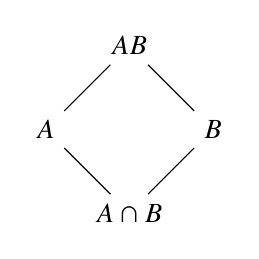
\begin{tikzpicture}[scale=1, node distance=1.5cm]
           \node (AB) {$AB$};
           \node [below left of=AB] (A) {$A$};
           \node [below right of=AB] (B) {$B$};
           \node [below left of=B] (AcapB) {$A \cap B$};
           \draw (AB) -- (A) -- (AcapB) -- (B) -- (AB);
      \end{tikzpicture}
 \end{center}

\vspace*{\stretch{1}}
\end{flashcard}


\begin{flashcard}[Groups]{State the \underline{Third Isomorphism Theorem} for groups}
\vspace*{\stretch{1}}
 Let $G$ be a group and let $H,K$ be normal subgroups of $G$ with $H \leq K$. Then $K/H \trianglelefteq G/H$ and $(G/H)/(K/H) \cong G/K$.
\vspace*{\stretch{1}}
\end{flashcard}

\begin{flashcard}[Groups]{State the \underline{Fourth (Lattice) Isomorphism Theorem} for groups}
\vspace*{\stretch{1}}
 Let $G$ be a group and let $N$ be a normal subgroup of $G$. Then there is a bijection from the set of subgroups $A$ of $G$ which contain $N$ onto the set of subgroups $\overline{A} = A/N$ of $G/N$.
\vspace*{\stretch{1}}
\end{flashcard}

\begin{flashcard}[Groups]{State the definition of a \underline{composition series}.}
\vspace*{\stretch{1}}
 Let $G$ be a group. Then a composition series is a sequence of subgroups
 $$
 1 = N_0 \leq N_1 \leq N_2 \leq \cdots \leq N_{k-1} \leq N_k = G
 $$
 such that $N_i \trianglelefteq N_{i+1}$ and $N_{i+1}/N_i$ is a simple group. The quotients $N_{i+1}/N_i$ are called \emph{composition factors} of $G$.
\vspace*{\stretch{1}}
\end{flashcard}

\begin{flashcard}[Groups]{What does it mean for a group to be \underline{solvable?}}
\vspace*{\stretch{1}}
 A group $G$ is solvable if there is a chain of subgroups
 $$
 1 = G_0 \trianglelefteq G_1 \trianglelefteq G_2 \trianglelefteq \cdots \trianglelefteq G_s = G
 $$
 such that $G_{i+1}/G_i$ is abelian.
\vspace*{\stretch{1}}
\end{flashcard}

\begin{flashcard}[Groups]{Prove that $p$-groups are solvable.}
\vspace*{\stretch{1}}
 A $p$-group has a normal subgroup for every divisor of its order, so we can form a chain of normal subgroups each of index $p$ relative to the group above it. Then each quotient is of order $p$ and thus abelian. This mean the $p$-group is solvable.
\vspace*{\stretch{1}}
\end{flashcard}

\begin{flashcard}[Groups]{$G$ is a group, $H \leq G$. Let $G$ act by left multiplication on the set $A$ of left cosets of $H$. Let $\pi_H$ be the permutation representation.\\
\vspace*{1pt}
(1) True or False: $G$ acts transitively on $A$.\\
(2) What is the stabilizer of the point $1H \in A$?\\
(3) What is the kernel of the action of $\pi_H$?}
\vspace*{\stretch{1}}
 \begin{enumerate}
      \item True
      \item $H$ is the stabilizer in $G$ of the point $1H$
      \item The kernel of $\pi_H$ is $\displaystyle \bigcap_{x \in G} x H x \inv$. This kernel is the largest normal subgroup of $G$ contained in $H$.
 \end{enumerate}
\vspace*{\stretch{1}}
\end{flashcard}

\begin{flashcard}[Groups]{State \underline{Cayley's Theorem}.}
\vspace*{\stretch{1}}
 Every group is isomorphic to a subgroup of some symmetric group. If $G$ is a group of order $n$, then $G$ is isomorphic to a subgroup os $S_n$.
\vspace*{\stretch{1}}
\end{flashcard}

\begin{flashcard}[Groups]{If $G$ is a finite group of order $n$ and $p$ is the smallest prime dividing $|G|$, then what can we say about a subgroup $H$ whose index is $p$?}
\vspace*{\stretch{1}}
 $H$ is normal in $G$.
\vspace*{\stretch{1}}
\end{flashcard}

\begin{flashcard}[Groups]{For some subset $S$ of a group $G$, how many conjugates of $S$ are there? Use the normalizer $N_G(S)$ in your answer.}
\vspace*{\stretch{1}}
 The number of conjugates of a subset $S$ is the index of the normalizer of $S$, $|G:N_G(S)|$. In particular, the number of conjugates of an element $S$ of $G$ is the index of the centralizer of $s$, $|G:C_G(s)|$.
\vspace*{\stretch{1}}
\end{flashcard}

\begin{flashcard}[Groups]{State and explain the \underline{class equation}.}
\vspace*{\stretch{1}}
 Let $G$ be a finite group. Then
 $$
 |G| = |Z(G)| + \sum_{i=1}^r |G: C_G(g_i)|
 $$
 where $Z(G)$ is the center of $G$ and each $g_i$ is a representative from a conjugacy class of $G$ not contained in $Z(G)$.
\vspace*{\stretch{1}}
\end{flashcard}

\begin{flashcard}[Groups]{How many conjugacy classes of $S_n$ are there?}
\vspace*{\stretch{1}}
 The number of conjugacy classes of $S_n$ is equal to the number of partitions of $n$. Also note that two elements of $S_n$ are conjugate if and only if they have the same cycle type.
\vspace*{\stretch{1}}
\end{flashcard}

% 
% \begin{flashcard}[Groups]{Let $H$ be a subgroup of $G$. If $H$ is normal, what can we say about $g H g \inv$ for all $g \in G$? What can we say about $g H g \inv$ if $H$ is not normal?}
% \vspace*{\stretch{1}}
%  If $H$ is normal, then conjugation by $g$ is an automorphism of $H$. The permutation representation afforded by this action is a homomorphism of $G$ into $\Aut(H)$ with kernel $C_G(H).$\\
%  
%  If $H$ is not normal, then (page 134, corollary 14: what? this seems to be the same.)
% \vspace*{\stretch{1}}
% \end{flashcard}


\begin{flashcard}[Groups]{Complete this sentence:\\ \vspace{5pt} Group $H$ is isomorphic to a subgroup of group $G$ if and only if there exists a \blank homomorphism from $H$ to $G$.}
\vspace*{\stretch{1}}
 injective
\vspace*{\stretch{1}}
\end{flashcard}

\begin{flashcard}[Groups]{Name two different methods for writing $(1 \; 2 \; 3 \; 4)$ as a product of transpositions.}
\vspace*{\stretch{1}}
 \emph{Head-to-Tail method: } $(1 \; 4) \; (1 \; 3) \; (1 \; 2)$\\
 
 \emph{Swap-the-Last-to-First method: } $(1 \; 2) \; (2 \; 3) \; (3 \; 4)$
\vspace*{\stretch{1}}
\end{flashcard} 

\begin{flashcard}[Groups]{State the definition of a \underline{characteristic} subgroup.}
\vspace*{\stretch{1}}
 A subgroup $H$ of a group $G$ is \emph{characteristic} if every automorphism of $G$ maps $H$ to itself.
\vspace*{\stretch{1}}
\end{flashcard} 

\begin{flashcard}[Groups]{Let $G$ be a group and $H$ be a subgroup. What is the relationship between $H$ and $gH g \inv$ for any element $g \in G$? What is the relationship if $H$ is normal?}
\vspace*{\stretch{1}}
 $H$ is always isomorphic to $g H g \inv.$ If $H$ is normal, then conjugation by $g$ is an automorphism of $H$.
\vspace*{\stretch{1}}
\end{flashcard} 

\begin{flashcard}[Groups]{Let $G$ be a group and $H$ be a subgroup. Let $G$ act on $H$ by conjugation. What is the kernel of the permutation representation of $G$ afforded by this group action?}
\vspace*{\stretch{1}}
 The permutation representation afforded by this action of $g$ on $H$ is a homomorphism of $G$ into $\Aut(H)$ with kernel $C_G(H).$
\vspace*{\stretch{1}}
\end{flashcard} 

\begin{flashcard}[Groups]{If $K$ is a characteristic subgroup of $H$ and $H$ is a normal subgroup of $G$. What can we say about $K$ relative to $G$?}
\vspace*{\stretch{1}}
 $K$ is normal in $G$.
\vspace*{\stretch{1}}
\end{flashcard} 

\begin{flashcard}[Groups]{What is the isomorphism type of $\Aut(G)$ if $G$ is cyclic of order $n$? What is the order of $\Aut(G)$?}
\vspace*{\stretch{1}}
 $\Aut(G) \cong (\Z/n\Z)^\times$, which is of order $\phi(n)$ where $\phi$ is the totient function.\\
 
 $\Aut(G)$ is isomorphic to the units of $\Z/n\Z$ because an automorphism of $G$ is uniquely determined by mapping any generator to any other generator.
\vspace*{\stretch{1}}
\end{flashcard}

\begin{flashcard}[Groups]{What is the order of the automorphism group of $\Z/n\Z$ when $n$ is a prime? What if $n$ is not prime?}
\vspace*{\stretch{1}}
 In both cases, the order of the automorphism group if $\phi(n)$ where $\phi$ is the totient function. \\
 
 If $n = p$ is a prime, then $\Aut(\Z/p/Z) \cong \Z/(p-1)\Z$.\\
 
 If $n = p_1^{e_1} \cdots p_k^{e_k}$, then $\Z/n\Z^\times \cong (\Z/p_1^{e_1} \Z)^\times  \times \cdots \times (\Z/p_k^{e_k} \Z)^\times$ by Chinese Remainder Theorem or structure theorem for modules over PIDs.
\vspace*{\stretch{1}}
\end{flashcard}

\begin{flashcard}[Groups]{What is isomorphism type of the automorphism group of $(\Z/p\Z)^n$?}
\vspace*{\stretch{1}}
 $\Aut((\Z/p\Z)^n) = GL_n(\Z/p\Z)$ \\
 
 $\{ (1, 0, \ldots, 0), (0, 1, 0, \ldots, 0), \ldots, (0, \ldots, 0, 1) \}$ is a basis for $(\Z/p\Z)^n$  as a vector space. Take any $\{v_1, \ldots , v_n\}$. By Linear algebra we have that the mapping $T(e_i) = v_i$ extends uniquely to a linear transformation of $V$. Each such $T$ is a group endomorphism from $V$ to $V$ and likewise any endomorphism of $V$ is a linear map of $V$ as a vector space. If we restrict our attention to automorphisms of $V$ we have $\Aut(V) = \{ T : V \to V \mid \ker T = 0 \} = GL_n(\Z/p\Z)$.
\vspace*{\stretch{1}}
\end{flashcard}

\begin{flashcard}[Groups]{What is the isomorphism type of $\Aut(D_8)$?}
\vspace*{\stretch{1}}
 $\Aut(D_8) \cong D_8$
\vspace*{\stretch{1}}
\end{flashcard}

\begin{flashcard}[Groups]{What is the isomorphism type of $\Aut(Q8)$?}
\vspace*{\stretch{1}}
 $\Aut(Q_8) \cong S_4$
\vspace*{\stretch{1}}
\end{flashcard}

\begin{flashcard}[Groups]{Suppose $n$ is a positive integer but $n \neq 6$.\\ What is the isomorphism type of $\Aut(S_n)$? \\ What is the index of $\Inn(S_n)$ in $\Aut(S_n)$?}
\vspace*{\stretch{1}}
 For all $n \neq 6$, $\Aut(S_n) \cong S_n$.\\
 
Symmetric groups aside from $S_6$ have only inner automorphisms, so $\Aut(S_n) = \Inn(S_n)$ and the index of $\Inn(S_n)$ in $\Aut(S_n)$ is 1.
\vspace*{\stretch{1}}
\end{flashcard}

\begin{flashcard}[Groups]{State \underline{Sylow's Theorem}.}
\vspace*{\stretch{1}}
 Let $G$ be a group of order $p^\alpha m$, $p \nmid m$. Let $n_p = |Syl_p(G)|$.
 \begin{enumerate}
      \item If $P \in Syl_p(G)$ and $Q$ is any $p$-subgroup, then $Q$ is a subgroup of some conjugate of $P$.
      \item $n_p \equiv 1 \mod p$.
      \item $n_p \mid m.$ This is because $n_p = [G:N_G(P)]$
 \end{enumerate}
\vspace*{\stretch{1}}
\end{flashcard}

\begin{flashcard}[Groups]{Let $P$ be a normal Sylow $p$-subgroup of $G$. What is the image of $P$ under any element of $\Aut(G)$? How many other Sylow $p$-subgroups besides $P$ are there?}
\vspace*{\stretch{1}}
 The image of $P$ under an automorphism of $G$ is just $P$ itself. This is because normal Sylow $p$-subgroups are characteristic.\\
 
 There are no other Sylow $p$-subgroups besides $P$. Conjugation by elements of $G$ induces a transitive action on the set of Sylow $p$-subgroups, so if $P$ is normal, there are no other Sylow $p$-subgroups.
\vspace*{\stretch{1}}
\end{flashcard}

\begin{flashcard}[Groups]{For what values of $n$ is $A_n$ a simple group?}
\vspace*{\stretch{1}}
 For $n \not=4$.
\vspace*{\stretch{1}}
\end{flashcard}

\begin{flashcard}[Groups]{State the \underline{Fundamental Theorem of} \underline{Finitely Generated Abelian Groups}.}
\vspace*{\stretch{1}}
 Let $G$ be a finitely generated abelian group. Then
 \begin{enumerate}
      \item $G \cong \Z^r \times \Z_{n_1} \times \Z_{n_2} \times \cdots \times \Z_{n_s}$ for integers $r, n_1, \ldots, n_s$ such that $r \geq 0$, $n_j \geq 2$ for all $j$, and $n_{i+1} \divides n_i$ for all $1 \leq i \leq s-1$ and
      \item the expression in (1) is unique
 \end{enumerate}
\vspace*{\stretch{1}}
\end{flashcard}

\begin{flashcard}[Groups]{Determine all possible abelian groups of order 180 by using invariant factors}
\vspace*{\stretch{1}}
 $180 = 2^2 \cdot 3^2 \cdot 5$, so the possible invariant factors (and the corresponding abelian groups) are listed below:
 \begin{center} $\begin{array}{c|c}
      \text{Invariant factors} & \text{Abelian Groups} \\
      \hline
      2^2 \cdot 3^2 \cdot 5 & \Z_{180} \\
      2 \cdot 3^2 \cdot 5, 2 & \Z_{90} \times \Z_2 \\
      2^2 \cdot 3 \cdot 5, 3 & \Z_{60} \times \Z_3 \\
      2 \cdot 3 \cdot 5, 2 \cdot 3 & \Z_{30} \times \Z_6 \\
 \end{array}$ \end{center}
\vspace*{\stretch{1}}
\end{flashcard}

\begin{flashcard}[Groups]{Describe the process of obtaining elementary divisors from invariant factors. \\ \vspace{5pt} Then describe the process of obtaining invariant factors from elementary divisors.}
\vspace*{\stretch{1}}
 \emph{Invariant factors to elementary divisors: } Factor each invariant factor into prime powers. This list of prime powers are the elementary divisors.\\
 
 \emph{Elementary divisors to invariant factors: } Group together the elementary divisors that are powers of the same prime. The largest invariant factor is the product of highest power primes in each group. The second invariant factor is the product of second-highest power primes in each group, and so on.
\vspace*{\stretch{1}}
\end{flashcard}

\begin{flashcard}[Groups]{Table of Groups of Small Order: List all groups of order $n$ for $n \in \{1, 2, 3, 4, 5\}$}
\vspace*{\stretch{1}}
 All of these groups are cyclic.
 {\def\arraystretch{1.5}
 \begin{center} $\begin{array}{c|c}
      \text{Order} & \text{Group} \\
      \hline
      1 & \Z_1 \\
      2 & \Z_2 \\
      3 & \Z_3 \\
      4 & \Z_4, \Z_2 \times \Z_2 \\
      5 & \Z_5
 \end{array}$ \end{center} }
\vspace*{\stretch{1}}
\end{flashcard}

\begin{flashcard}[Groups]{Table of Groups of Small Order: List all groups of order $n$ for $n \in \{6, 7, 8, 9, 10\}$}
\vspace*{\stretch{1}}
{\def\arraystretch{1.5}
 \begin{center} $\begin{array}{c|c}
      \text{Order} & \text{Group} \\
      \hline
      6 & \Z_6, S_3 \\
      7 & \Z_7 \\
      8 & \Z_8, \Z_4 \times \Z_2, \Z_2^2, D_8, Q_8 \\
      9 & \Z_9, \Z_3^2 \\
      10 & \Z_{10}, D_{10}
 \end{array}$ \end{center} }
\vspace*{\stretch{1}}
\end{flashcard}

\begin{flashcard}[Groups]{Table of Groups of Small Order: List all groups of order $n$ for $n \in \{11, 12, 13, 14, 15 \}$}
\vspace*{\stretch{1}}
 {\def\arraystretch{1.5}
 \begin{center} $\begin{array}{c|c}
      \text{Order} & \text{Group} \\
      \hline
      11 & \Z_{11} \\
      12 & \Z_{12}, \Z_{6} \times \Z_{2}, A_4, D_{12}, \Z_{3} \rtimes \Z_{4} \\
      13 & \Z_{13} \\
      14 & \Z_{14}, D_{14} \\
      15 & \Z_{15} \\
 \end{array}$ \end{center} }
\vspace*{\stretch{1}}
\end{flashcard}

\begin{flashcard}[Groups]{Table of Groups of Small Order: List all abelian groups of order 16. List 3 non-abelian groups of order 16.}
\vspace*{\stretch{1}}
 \emph{Abelian groups: } $\Z_{16}, \Z_8 \times \Z_2, \Z_4 \times \Z_4, \Z_4 \times \Z_2 \times \Z_2, \Z_2^4$\\
 
 \emph{Non-abelian groups: } $D_{16}, D_{8} \times \Z_2, Q_8 \times \Z_2$
\vspace*{\stretch{1}}
\end{flashcard}

\begin{flashcard}[Groups]{Table of Groups of Small Order: List all groups of order $n$ for $n \in \{17, 18, 19, 20 \}$}
\vspace*{\stretch{1}}
 {\def\arraystretch{1.5}
 \begin{center} $\begin{array}{c|c}
      \text{Order} & \text{Group} \\
      \hline
      17 & \Z_{17} \\
      18 & \Z_{18}, \Z_6 \times \Z_3, D_{18}, S_3 \times \Z_3, \Z_3^2 \rtimes \Z_2 \\
      19 & \Z_{19} \\
      20 & \Z_{20}, \Z_{10} \times \Z_2, D_{20}, \Z_5 \rtimes \Z_4, F_{20}
 \end{array}$ \end{center} }
 \emph{Note: }$F_{20} = \langle x,y \mid x^4 = y^5 = 1, xyx \inv = y^2 \rangle$
\vspace*{\stretch{1}}
\end{flashcard}

\begin{flashcard}[Groups]{Classify all groups of order $pq$ when $p,q$ are distinct primes.}
\vspace*{\stretch{1}}
 Assume $p > q$. \\
 
 If $p \nmid q-1$, the only possible group is the cyclic group of order $pq$.\\
 
 If $p \divides q-1$, then there are two possible groups: the cyclic group of order $pq$ and the semidirect product $\Z_q \rtimes \Z_p$.
\vspace*{\stretch{1}}
\end{flashcard}

\begin{flashcard}[Groups]{Let $G$ be a group and let $x,y \in G$. What is $[x,y]$, the \underline{commutator} of $x$ and $y$? Why is it called a commutator?}
\vspace*{\stretch{1}}
 $[x,y] = x \inv y \inv x y$\\
 
 This is called a commutator because $xy = yx[x,y]$
\vspace*{\stretch{1}}
\end{flashcard}

\begin{flashcard}[Groups]{What is a \underline{commutator subgroup} of a group $G$? Is it a normal subgroup? If so, what can we say about the quotient of $G$ by the commutator subgroup?}
\vspace*{\stretch{1}}
 The commutator subgroup $[G,G]$ of group $G$ is defined as $\langle [x,y] = x \inv y \inv x y \mid x,y \in G \rangle$. It is a normal subgroup of $G$ and quotienting by it gives an abelian group. In fact, $G/[G,G]$ is the largest abelian quotient in the sense that if $H \trianglelefteq G$ and $G/H$ is abelian, then $[G,G] \leq H$.
\vspace*{\stretch{1}}
\end{flashcard}

\begin{flashcard}[Groups]{What factoring property does the map $G \to G/[G,G]$ have?}
\vspace*{\stretch{1}}
 If $A$ is an abelian group and $\phi: G \to A$ is a homomorphism, then $\phi$ factors through $[G,G]$ and the following diagram commutes:
 \begin{center}
      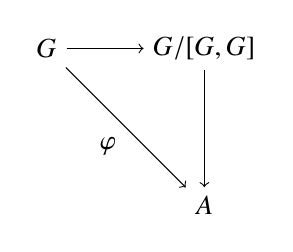
\begin{tikzpicture}[node distance=2cm]
           \node (G) {$G$};
           \node [right of=G] (quotient) {$G/[G,G]$};
           \node [below of=quotient] (A) {$A$};
           \draw [->] (G) -- (quotient);
           \draw [->] (quotient) -- (A);
           \draw [->] (G) -- (A);
           \node [below left] at (1,-1) {$\phi$};
      \end{tikzpicture}
 \end{center}
\vspace*{\stretch{1}}
\end{flashcard}

\begin{flashcard}[Groups]{What is the universal property of the abelianization?}
\vspace*{\stretch{1}}
 \emph{Note: }This is the same answer as ``What factoring property does the map $G \to G/[G,G]$ have?''\\
 
  If $A$ is an abelian group and $\phi: G \to A$ is a homomorphism, then $\phi$ factors through $[G,G]$ and the following diagram commutes:
 \begin{center}
      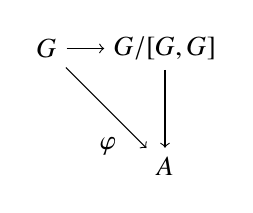
\begin{tikzpicture}[node distance=1.5cm]
           \node (G) {$G$};
           \node [right of=G] (quotient) {$G/[G,G]$};
           \node [below of=quotient] (A) {$A$};
           \draw [->] (G) -- (quotient);
           \draw [->] (quotient) -- (A);
           \draw [->] (G) -- (A);
           \node [below left] at (1,-1) {$\phi$};
      \end{tikzpicture}
 \end{center}
\vspace*{\stretch{1}}
\end{flashcard}

\begin{flashcard}[Groups]{Prove that $[G,G] \trianglelefteq G$}
\vspace*{\stretch{1}}
 Let $g \in G$. Then $g [G,G] g \inv = g \langle [x,y] \mid x,y \in G \rangle g \inv = \langle g[x,y]g \inv \mid x,y \in G \rangle = \langle [gxg \inv,gyg \inv] \mid x,y \in G \rangle = \langle [x,y] \mid x,y \in G \rangle$, with the last equality holding since conjugation is an automorphism on $G$.
\vspace*{\stretch{1}}
\end{flashcard}

\begin{flashcard}[Groups]{State the recognition theorem for the direct and semidirect product of groups.}
\vspace*{\stretch{1}}
 \emph{Direct Product:} If group $G$ contains normal subgroups $H$ and $K$, $H \cap K$ = 1, and $G = HK$, then $G \cong H \times K$. \\
 
 \emph{Semidirect Product:} The conditions are the same as above, but only one subgroup needs to be normal.
\vspace*{\stretch{1}}
\end{flashcard}

\begin{flashcard}[Groups]{True or False: Every group can be written as a semidirect product. Give a proof or counterexample.}
\vspace*{\stretch{1}}
 False. $Q_8$ is not a semidirect product because no two subgroups have trivial intersection. Every subgroup contains the subgroup $\{1, -1\}$. 
\vspace*{\stretch{1}}
\end{flashcard}

\begin{flashcard}[Groups]{List all groups of order $p^3$.}
\vspace*{\stretch{1}}
 The three abelian groups are $\Z_{p^3}$, $\Z_{p^2} \times \Z_p$, and $\Z_p^3$.\\
 
%  One of the two non-abelian groups is $\Z_{p^2} \rtimes \Z_p$. If $p=2$, this is $D_8$.  If $p \neq 2$, this is the Heisenberg group
 $$\Heis(\F_p) = \left \{ \left ( {\def\arraystretch{.5} \begin{array}{ccc}
1 & a & b \\
0 & 1 & c \\
0 & 0 & 1                                                                                                                                                                             \end{array} } \right ) : a,b,c \in \F_p \right \}.$$
\vspace{5pt}
If $p=2$, this last group is $Q_8$. If $p \neq 2$, the last group is some group of exponent $p$.
\vspace*{\stretch{1}}
\end{flashcard}

\begin{flashcard}[Groups]{If every group of order $n$ (for some particular $n$) can be expressed as a semidirect product, what steps do you take to classify all groups of order $n$?}
\vspace*{\stretch{1}}
 \begin{enumerate}
      \item Show every group $G$ of order $n$ has proper subgroups $H,K$ such that $H \trianglelefteq G$, $H \cap K = 1$ and $HK = G$
      \item Find all possible isomorphism types for $H$ and $K$
      \item For each pair $H,K$ found in (2), find all possible homomorphisms $\phi: K \to \Aut(H)$
      \item For each triple $H,K,\phi$ found in (3), form the semidirect product $H \rtimes_{\phi} K$ and determine which ones are isomorphic
 \end{enumerate}
\vspace*{\stretch{1}}
\end{flashcard}

\begin{flashcard}[Groups]{Suppose group $G$ can be expressed as a semidirect product $H \rtimes K$. \\ If $(h_1, k_1), (h_2, k_2) \in G$, what is $(h_1, k_1)(h_2, k_2)$? (That is, how is the group operation defined in a semidirect product?)}
\vspace*{\stretch{1}}
 $(h_1, k_1)(h_2, k_2) = (h_1 (k_1 \cdot h_2), k_1 k_2)$ where $k_1 \cdot h_2$ is the action of $k_1$ on $h_2$ as defined by $\phi$, some automorphism of $H$.
\vspace*{\stretch{1}}
\end{flashcard}

\begin{flashcard}[Groups]{List the properties of $p$-groups.}
\vspace*{\stretch{1}}
Let $P$ be a group whose order is $p^a$ for prime $p$.
 \begin{enumerate}
      \item The center of $P$ is nontrivial.
      \item If $H$ is a nontrivial normal subgp, then it intersects the center nontrivially.
      \item $P$ has a normal subgp of any order dividing $p^a$.
      \item Every proper subgp of $P$ is a proper subgp of its normalizer in $P$. (i.e. nilpotent)
      \item Every maximal subgp has index $p$ and is normal in $P$.
      \item $P$ is nilpotent of nilpotence class at most $a-1$.
 \end{enumerate}
\vspace*{\stretch{1}}
\end{flashcard}

\begin{flashcard}[Groups]{What is an \underline{upper central series}?}
\vspace*{\stretch{1}}
 The \emph{upper central series} for a group $G$ is the chain of subgroups
 $$
 Z_0(G) \leq Z_1(G) \leq Z_2(G) \leq \cdots
 $$
 where the subgroups are inductively defined as $Z_0(G) = 1$, $Z_1(G) = Z(G)$, and $Z_{i+1}(G)$ is the subgroup of $G$ containing $Z_i(G)$ such that $Z_{i+1}(G)/Z_i(G) = Z(G/Z_i(G))$
\vspace*{\stretch{1}}
\end{flashcard}

\begin{flashcard}[Groups]{What does it mean for a group to be \underline{nilpotent}? What is the \underline{nilpotence class} of a nilpotent group?}
\vspace*{\stretch{1}}
 A group $G$ is called \emph{nilpotent} if $Z_c(G) = G$ for some $c \in \Z$. The smallest such $c$ is the \emph{nilpotence class} of $G$.
\vspace*{\stretch{1}}
\end{flashcard}

\begin{flashcard}[Groups]{What is the nilpotence class of an abelian group?}
\vspace*{\stretch{1}}
 It is 1, since $Z_1(G) = Z(G) = G$.
\vspace*{\stretch{1}}
\end{flashcard}

\begin{flashcard}[Groups]{Arrange the following types of groups in a chain of inclusions: cyclic groups, nilpotent groups, solvable groups, abelian groups, all groups}
\vspace*{\stretch{1}}
 cyclic groups $\subseteq$ abelian groups $\subseteq$ nilpotent groups\\ $\subseteq$ solvable groups $\subseteq$ all groups
\vspace*{\stretch{1}}
\end{flashcard}

\begin{flashcard}[Groups]{Let $G$ be a finite group, let $p_1, \ldots, p_2$ be the distinct primes dividing its order, and let $P_i \in Syl_{p_i}(G)$, $1 \leq i \leq s$. State 5 conditions that are equivalent to the nilpotence of $G$.}
\vspace*{\stretch{1}}
 \begin{enumerate}
      \item If $H < G$, then $H < N_G(H)$ (``normalizer grows'')
      \item $P_i \trianglelefteq G$ for $1 \leq i \leq s$ (every Sylow subgroup is normal)
      \item $G \cong P_1 \times P_2 \times \cdots \times P_s$
      \item Every maximal subgroup of $G$ is normal
      \item Its central series (or lower/upper central series) terminates after finitely many steps.
 \end{enumerate}
\vspace*{\stretch{1}}
\end{flashcard}

\begin{flashcard}[Groups]{What is a \underline{lower central series}?}
\vspace*{\stretch{1}}
 For a group $G$, the \emph{lower central series} is the chain of subgroups
 $$
 G^0 \geq G^1 \geq G^2 \geq \cdots
 $$
 where the subgroups are defined inductively as $G^0 = G$, $G^1 = [G,G]$, and $G^{i+1} = [G, G^{i}]$.
\vspace*{\stretch{1}}
\end{flashcard}

\begin{flashcard}[Groups]{What is the \underline{derived series} or \underline{commutator series} of a group $G$?}
\vspace*{\stretch{1}}
 The \emph{derived} or \emph{commutator series} of a group $G$ is the following sequence of groups, defined inductively $\forall i \geq 1$.
 $$
 G^{(0)} = G \qquad G^{(1)} = [G,G] \qquad G^{(i+1)} = [G^{(i)}, G^{(i)}]
 $$
\vspace*{\stretch{1}}
\end{flashcard}

\begin{flashcard}[Groups]{For a group $G$, what condition on the groups in the derived series of $G$ is necessary and sufficient for $G$ to be solvable?}
\vspace*{\stretch{1}}
 $G$ is solvable if and only if $G^{(n)} = 1$ for some $n \geq 0$.
\vspace*{\stretch{1}}
\end{flashcard}

\begin{flashcard}[Groups]{State Burnside's theorem on groups of order $p^aq^b$.}
\vspace*{\stretch{1}}
 Such groups are solvable.
\vspace*{\stretch{1}}
\end{flashcard}


\begin{flashcard}[Groups]{(Techniques for producing normal subgroups in groups of order $n$) \\ \vspace{5pt} Describe the technique known as ``counting elements.''}
\vspace*{\stretch{1}}
 Use this technique when for $P \in Syl_p(G)$, $|P| = p$.\\
 
 Suppose by contradiction the group is simple so that the number of Sylow $p$-subgroups is greater than 1 (i.e. $n_p > 1$). Since each Sylow $p$-subgroup intersects only at the identity, count the number of elements in each subgroup. If the total elements counted is greater than $n$, then at least one $n_p$ must be 1 and the unique Sylow $p$-subgroup is normal.
\vspace*{\stretch{1}}
\end{flashcard}

\begin{flashcard}[Groups]{(Techniques for producing normal subgroups in groups of order $n$) \\ \vspace{5pt} Describe the technique known as ``exploiting subgroups of small index.''}
\vspace*{\stretch{1}}
 Let $|G| = n$, $H \leq G$, $[G:H] = k$. $G$ acting on cosets of $H$ by left multiplication induces a map from $G$ to $S_k$. Suppose $G$ is simple so that the kernel is trivial. Then $G$ is isomorphic to a subgroup of $S_k$ so $n \divides k!$. Because of this argument, if $k$ is the smallest integer such that $n \divides k!$, then $\nexists$ $H < G$ with index less than $k$.\\
 
 ex) Suppose $n = 3993 = 3^2 \cdot 13 \cdot 29$. The possible indices of a subgroup are $3, 9, 13, \ldots.$ Of these, only 29! is divisible by 3993.
\vspace*{\stretch{1}}
\end{flashcard}

\begin{flashcard}[Groups]{(Techniques for producing normal subgroups in groups of order $n$) \\ \vspace{5pt} Describe the technique known as ``permutation representations."}
\vspace*{\stretch{1}}
 Let $|G| = n$ and $H$ a subgroup of index $k$. Let $\phi: G \to S_k$ be the permutation representation of $G$ by action on cosets of $H$. Suppose that $G$ is simple. Then the kernel is trivial and $G$ is isomorphic to a subgroup of $S_k$. We can attempt to show that $S_k$ contains no simple subgroup of order $n$.\\
 
 We can use facts such as (1) if $G$ contains an element/subgp of some order, so must $S_k$ and (2) if $P \in Syl_p(G)$ and $P \in Syl_p(S_k)$, then $|N_G(P)|$ divides $|N_{S_k}(P)|$.
\vspace*{\stretch{1}}
\end{flashcard}

\begin{flashcard}[Groups]{(Techniques for producing normal subgroups in groups of order $n$) \\ \vspace{5pt} Describe the technique known as ''playing $p$-subgroups against each other for different primes $p$.``}
\vspace*{\stretch{1}}
 This technique is for primes $p,q$ such that $p<q$ and $p \nmid q-1$ (this makes groups of order $pq$ cyclic).\\
 
 If $G$ has a Sylow $q$-subgroup $Q$ of order $q$ and $p \divides | N_G(Q) |$, then Cauchy's Theorem says $P = \langle p \rangle$ is a group of order $p$ that normalizes $Q$. Then $PQ$ is cyclic and thus abelian, so $PQ \leq N_G(P)$ and $q \divides |N_G(P)|$. This may force $N_G(P) = G$ or may force the index of $N_G(P)$ to be lower than that which is allowable by the ''exploiting subgroups of small index`` technique.
\vspace*{\stretch{1}}
\end{flashcard}

\begin{flashcard}[Groups]{(Techniques for producing normal subgroups in groups of order $n$) \\ \vspace{5pt} Describe the technique known as ''studying normalizers of intersections of Sylow $p$-subgroups.``}
\vspace*{\stretch{1}}
 Suppose $R,P \in Syl_p(G)$ are distinct subgroups and $R \cap P \neq 1$. Then by property 4 in the list of properties of $p$-groups, $P_0 = R \cap P$ satisfies $P_0 < N_P(P_0)$ and $P_0 < N_R(P_0)$. This may cause the normalizer in $G$ of $P_0$ to have too small an index to satisfy the bound provided by the ''exploiting subgroups of small index`` technique.
\vspace*{\stretch{1}}
\end{flashcard}

\begin{flashcard}[Groups]{What is the universal property of the free group $F(S)$ on a set $S$?}
\vspace*{\stretch{1}}
 Any map from set $S$ to a group $G$ extends uniquely to a homomorphism $\phi$ from $F(S)$ to $G$.
 \begin{center}
      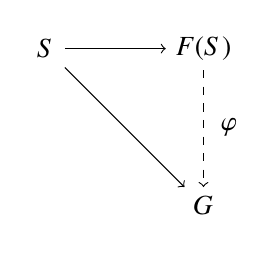
\begin{tikzpicture}[node distance = 2cm]
           \node (S) {$S$};
           \node [right of=S] (F) {$F(S)$};
           \node [below of=F] (G) {$G$};
           \draw [->] (S) -- (G);
           \draw [->] (S) -- (F);
           \draw [->, dashed] (F) -- (G);
           \node [right] at (2.1,-1) {$\phi$};
      \end{tikzpicture}
 \end{center}
\vspace*{\stretch{1}}
\end{flashcard}

\begin{flashcard}[Groups]{What is a \underline{free group}?}
\vspace*{\stretch{1}}
 A free group is a group with no relations. Its elements are just the \emph{words} made by the generators in some set $S$.
\vspace*{\stretch{1}}
\end{flashcard}

\begin{flashcard}[Groups]{The derived series of a group terminates (every group in the chain is eventually trivial group 1) if and only if the group is \blank}
\vspace*{\stretch{1}}
 solvable
\vspace*{\stretch{1}}
\end{flashcard}

\begin{flashcard}[Groups]{If $G,H$ are solvable groups, which of the following are also solvable? The direct product $H \times G$? The semidirect product $H \rtimes G$? Any subgroup $K$ of $G$? The quotient $G/N$ for some normal subgroup $N$ of $G$?}
\vspace*{\stretch{1}}
 These are all solvable. Ha!
\vspace*{\stretch{1}}
\end{flashcard}

\begin{flashcard}[Groups]{Let $a$ be an element of order $n$ and $b$ be an element of order $m$. Is it true that $\langle a, b \rangle$ has order $\lcm(a,b)$?}
\vspace*{\stretch{1}}
 No, this is not generally true. If the permutation representations of $a$ and $b$ are disjoint, then it is true.
\vspace*{\stretch{1}}
\end{flashcard}



\begin{flashcard}[Groups]{State and prove Frattini's Argument.}
\vspace*{\stretch{1}}
 If $H \trianglelefteq G$ and $P \in Syl_p(H)$, then $G = N_G(P)H$\\
 
 \emph{Proof: } Let $g \in G$. Then $g \inv P g \in H$ since $H \trianglelefteq G$. Thus $g \inv P g$ is also a Sylow $p$-subgroup of $H$. Since all Sylow $p$-subgroups of $H$ must be conjugate by some element of $H$, there exists $h \in H$ such that
 $$ h (g \inv P g) h \inv = P.$$
 So $g h \inv \in N_G(P)$ and $g \in N_G(P)H$. Since $g$ was arbitrary, $G \subseteq N_G(P)H$ which implies $G = N_G(P)H.$
\vspace*{\stretch{1}}
\end{flashcard}


\begin{flashcard}[Groups]{Prove that if $G$ is solvable, then $G/N$ is solvable.}
\vspace*{\stretch{1}}
 $G$ is a composition series such that each successive quotient is abelian. Quotienting every group in the series produces a composition series for $G/N$ such that each successive quotient is abelian. Thus $G/N$ is solvable. \vspace*{\stretch{1}}
\end{flashcard}


\begin{flashcard}[Groups]{Prove that if $N \trianglelefteq G$, $N$ is solvable, and $G/N$ is solvable, then $G$ is solvable.}
\vspace*{\stretch{1}}
 $N$ is solvable so there is composition series $1 = N_0 \trianglelefteq \cdots \trianglelefteq N_n = N$ so that $N_{i+1}/N_i$ is abelian. Likewise there is a series for $\overline{G} = G/N$ composed of subgroups $\overline{G_i}$. By the Lattice isomorphism theorem, there are subgroups $G_i$ of $G$ containing $N$ such that $G_i /N = \overline{G_i}$. Thus we can form the following composition series for $G$, each successive quotient is abelian, and $G$ is solvable:
 
 $$1 = N_0 \trianglelefteq \cdots \trianglelefteq N_n = N = G_0 \trianglelefteq \cdots \trianglelefteq G_m = G$$
\vspace*{\stretch{1}}
\end{flashcard}

% 
% \begin{flashcard}[topic]{front}
% \vspace*{\stretch{1}}
%  back
% \vspace*{\stretch{1}}
% \end{flashcard}
% 
% 
% \begin{flashcard}[topic]{front}
% \vspace*{\stretch{1}}
%  back
% \vspace*{\stretch{1}}
% \end{flashcard}
% 
% 
% \begin{flashcard}[topic]{front}
% \vspace*{\stretch{1}}
%  back
% \vspace*{\stretch{1}}
% \end{flashcard}
% 
% 
% \begin{flashcard}[topic]{front}
% \vspace*{\stretch{1}}
%  back
% \vspace*{\stretch{1}}
% \end{flashcard}
% 
% 
% \begin{flashcard}[topic]{front}
% \vspace*{\stretch{1}}
%  back
% \vspace*{\stretch{1}}
% \end{flashcard}
% 
% 
% \begin{flashcard}[topic]{front}
% \vspace*{\stretch{1}}
%  back
% \vspace*{\stretch{1}}
% \end{flashcard}
% 
% 
% \begin{flashcard}[topic]{front}
% \vspace*{\stretch{1}}
%  back
% \vspace*{\stretch{1}}
% \end{flashcard}
% 
% 
% \begin{flashcard}[topic]{front}
% \vspace*{\stretch{1}}
%  back
% \vspace*{\stretch{1}}
% \end{flashcard}
% 
% 
% \begin{flashcard}[topic]{front}
% \vspace*{\stretch{1}}
%  back
% \vspace*{\stretch{1}}
% \end{flashcard}
% 
% 
% \begin{flashcard}[topic]{front}
% \vspace*{\stretch{1}}
%  back
% \vspace*{\stretch{1}}
% \end{flashcard}
% 
% 
% \begin{flashcard}[topic]{front}
% \vspace*{\stretch{1}}
%  back
% \vspace*{\stretch{1}}
% \end{flashcard}
% 
% 
% \begin{flashcard}[topic]{front}
% \vspace*{\stretch{1}}
%  back
% \vspace*{\stretch{1}}
% \end{flashcard}
% 
% 
% \begin{flashcard}[topic]{front}
% \vspace*{\stretch{1}}
%  back
% \vspace*{\stretch{1}}
% \end{flashcard}
% 
% 
% \begin{flashcard}[topic]{front}
% \vspace*{\stretch{1}}
%  back
% \vspace*{\stretch{1}}
% \end{flashcard}
% 
% 
% \begin{flashcard}[topic]{front}
% \vspace*{\stretch{1}}
%  back
% \vspace*{\stretch{1}}
% \end{flashcard}
% 
% 
% \begin{flashcard}[topic]{front}
% \vspace*{\stretch{1}}
%  back
% \vspace*{\stretch{1}}
% \end{flashcard}
% 
% 
% \begin{flashcard}[topic]{front}
% \vspace*{\stretch{1}}
%  back
% \vspace*{\stretch{1}}
% \end{flashcard}

















%%%%% RINGS %%%%%


\begin{flashcard}[Rings]{What is a \underline{ring}?}
\vspace*{\stretch{1}}
 A \emph{ring} R is a set together with two binary operations $+$ and $\times$ such that
 \begin{enumerate}
      \item (R, +) is an abelian group
      \item $\times$ is associative
      \item The distributive property holds
 \end{enumerate}
\vspace*{\stretch{1}}
\end{flashcard}

\begin{flashcard}[Rings]{What is a \underline{division ring}? What is another name for a commutative division ring?}
\vspace*{\stretch{1}}
 A ring with identity ($1 \neq 0$) is a \emph{division ring} if every nonzero element has a multiplicative inverse.\\
 
 A commutative division ring is a \emph{field}.
\vspace*{\stretch{1}}
\end{flashcard}

\begin{flashcard}[Rings]{What is an \underline{integral domain}? What desirable property do integral domains possess? What desirable property do finite integral domains possess?}
\vspace*{\stretch{1}}
 An \emph{integral domain} is a ring with no zero divisors.\\
 
 Integral domains possess the cancellation property.\\
 
 Finite integral domains are fields.
\vspace*{\stretch{1}}
\end{flashcard}

\begin{flashcard}[Rings]{What is a \underline{left ideal}?}
\vspace*{\stretch{1}}
 Let $R$ be a ring, $I$ a subset of $R$, and $r \in R$. $I$ is an \emph{ideal} of $R$ if 
 \begin{enumerate}
      \item $I$ is a subring of $R$ and
      \item $I$ is closed under left multiplication by elements from $R$.
 \end{enumerate}
\vspace*{\stretch{1}}
\end{flashcard}

\begin{flashcard}[Rings]{What is the \underline{subring criterion}?}
\vspace*{\stretch{1}}
 Given any subset $S$ of a ring $R$, we know that $S$ is a subring if $S$ is nonempty and closed under subtraction and multiplication.
\vspace*{\stretch{1}}
\end{flashcard}

\begin{flashcard}[Rings]{What is a \underline{ring homomorphism}?}
\vspace*{\stretch{1}}
 Let $R,S$ be rings and $\phi: R \to S$. Then $\phi$ is a \emph{ring homomorphism} if $\phi(a+b) = \phi(a) + \phi(b)$ and $\phi(ab) = \phi(a) \phi(b)$.
\vspace*{\stretch{1}}
\end{flashcard}

\begin{flashcard}[Rings]{Is the kernel of a ring homomorphism an ideal of the domain?}
\vspace*{\stretch{1}}
 Yes indeedy.
\vspace*{\stretch{1}}
\end{flashcard}

\begin{flashcard}[Rings]{Let $I,J$ be ideals of ring $R$.\\ What is $I + J$? Is it an ideal of $R$?\\ What is $IJ$? Is it an ideal of $R$?}
\vspace*{\stretch{1}}
 $I+J = \{a+b \mid a \in I, b \in J\}$\\
 This is an ideal of $R$.\\
 
 $IJ = \{a_1b_1 + \cdots a_n b_n \mid a_1, \ldots, a_n \in I, b_1, \ldots, b_n \in J, n \in \Z^+\}$\\
 This is an ideal of $R$.\\
 
 Note: $S = \{ij \mid i \in I, j \in J \}$ is not necessarily an ideal.
\vspace*{\stretch{1}}
\end{flashcard}

\begin{flashcard}[Rings]{Let $I,J$ be ideals of ring $R$. Is it true that $I \cap J \subseteq IJ$?}
\vspace*{\stretch{1}}
 No. $IJ \subseteq I \cap J$. Sometimes $IJ$ may even be strictly smaller.
\vspace*{\stretch{1}}
\end{flashcard}

\begin{flashcard}[Rings]{Given a ring $R$ and some subset $A$, what is the ideal generated by $A$?}
\vspace*{\stretch{1}}
 The left ideal generated by $A$ is $$RA = \{r_1 a_1 + r_2 a_2 + \cdots + r_n a_n \mid r_i \in R, a_i \in A, n \in \Z^+ \}.$$
\vspace*{\stretch{1}}
\end{flashcard}

\begin{flashcard}[Rings]{Given a ring $R$ and ideal $I$, what is the condition that guarantees $I = R$?}
\vspace*{\stretch{1}}
  $I = R$ if and only if $I$ contains a unit\\
  
  \emph{Proof: } $(\rightarrow)$ If $I = R$, then $I$ contains 1, which is a unit.\\
  
  $(\leftarrow)$ If $a \in I$ is a unit, then $a \inv \in I$ as well. By the multiplicative sucking property, $a \inv a \in I$ and so $1 \in I$. Then every element of $R$ is in $I$ and $R = I$.
\vspace*{\stretch{1}}
\end{flashcard}

\begin{flashcard}[Rings]{If $R$ is a field, then what can we say about a nonzero ring homomorphism from $R$ to another ring?}
\vspace*{\stretch{1}}
 That homomorphism is injective. The kernel of the homomorphism would need to be an ideal, and the only ideals in a field are 0 and $R$. Since the homomorphism is nonzero, the kernel is not all of $R$. Thus the kernel is 0 and the map is injective.
\vspace*{\stretch{1}}
\end{flashcard}

\begin{flashcard}[Rings]{What is a \underline{maximal ideal}? Does every ring have maximal ideals? Which rings always have maximal ideals?}
\vspace*{\stretch{1}}
 An ideal $M$ in a ring $S$ is called a \emph{maximal ideal} if $M \neq S$ and the only ideals containing $M$ are $M$ and $S$.\\
 
 No, not every ring has maximal ideals. For example, $\Q$ equipped with standard addition and trivial multiplication ($ab = 0 \; \forall a,b \in \Q$) has no maximal ideals. We can perform this construction for any abelian group that has no maximal subgroups.\\
 
 In a ring with identity, every proper ideal is contained in a maximal ideal.
\vspace*{\stretch{1}}
\end{flashcard}

\begin{flashcard}[Rings]{Let $R$ be a ring and $I$. What can be said about $R/I$ when $I$ is maximal? What can be said about $R/I$ when $I$ is prime?}
\vspace*{\stretch{1}}
 $R/I$ is a field if and only if $I$ is a maximal ideal.\\
 
 $R/I$ is an integral domain if and only if $I$ is a prime ideal.
\vspace*{\stretch{1}}
\end{flashcard}

\begin{flashcard}[Rings]{What is a \underline{prime ideal}?}
\vspace*{\stretch{1}}
 Assume $R$ is a commutative ring. The ideal $P$ is a \emph{prime ideal} if $P \neq R$ and whenever $ab \in P$, at least one of $a$ or $b \in P$.
\vspace*{\stretch{1}}
\end{flashcard}

\begin{flashcard}[Rings]{In a commutative ring with unity, is every prime ideal a maximal ideal or is every maximal ideal a prime ideal? Give an example. In what kind of ring do prime and maximal ideals coincide?}
\vspace*{\stretch{1}}
 Every maximal ideal is a prime ideal. The converse is not always true: in any nonfield integral domain, the zero ideal is a prime ideal which is not maximal.\\
 
 In a PID, every nonzero prime ideal is maximal.
\vspace*{\stretch{1}}
\end{flashcard}

\begin{flashcard}[Rings]{Given a ring $R$, what is its \underline{ring of fractions}? Under what condition is the ring of fractions a field?}
\vspace*{\stretch{1}}
 Let $R$ be a commutative ring and $D$ a nonempty subset of $R$ that does not contain 0 or zero divisors and is closed under multiplication. Then the \emph{ring of fractions} is $Q = \left \{ \dfrac{r}{d} \mid r \in R, d \in D \right \}$.\\
 
 If $D = R - \{0\}$ (i.e. $R$ is an integral domain) then $Q$ is a field.
\vspace*{\stretch{1}}
\end{flashcard}

\begin{flashcard}[Rings]{Let $A,B$ be ideals in ring $R$. What does it mean for $A$ and $B$ to be \underline{comaximal}?}
\vspace*{\stretch{1}}
 Ideals $A$ and $B$ are \emph{comaximal} if $A+B=R$.
\vspace*{\stretch{1}}
\end{flashcard}

\begin{flashcard}[Rings]{State the Chinese Remainder Theorem. Give an example.}
\vspace*{\stretch{1}}
 Let $A_1, \ldots, A_k$ be ideals in ring $R$. The map $R \to R/A_1 \times \cdots \times R/A_k$ defined by $r \mapsto (r + A_1, \ldots, r + A_k)$ is a ring homomorphism with kernel $A_1 \cap \cdots \cap A_k$.\\
 
 If each pair of ideals in the list is comaximal, then this map is surjective and $A_1 \cap \cdots \cap A_k = A_1A_2 \cdots A_k$ so that $R/(A_1A_2 \cdots A_k) = R/(A_1 \cap \cdots \cap A_k) \cong R/A_1 \times \cdots \times R/A_k.$\\
 
 \emph{ex.)} If integer $n$ has prime factorization $p_1^{\alpha_1} \cdots p_k^{\alpha_k}$, then $\Z/n\Z \cong (\Z/p_1^{\alpha_1}\Z) \times \cdots \times (\Z/p_k^{\alpha_k}\Z)$ and $(\Z/n\Z)^\times \cong (\Z/p_1^{\alpha_1}\Z)^\times \times \cdots \times (\Z/p_k^{\alpha_k}\Z)^\times.$
\vspace*{\stretch{1}}
\end{flashcard}

\begin{flashcard}[Rings]{What is a \underline{Euclidean domain}?}
\vspace*{\stretch{1}}
 An integral domain $R$ is a \emph{Euclidean domain} if there exists a norm $N$ on $R$ such that for $a,b \in R$, there exist $q,r \in R$ such that
  $$
 a = qb + r \qquad \text{with }r=0 \text{ or }N(r) < N(b)
 $$
\vspace*{\stretch{1}}
\end{flashcard}

\begin{flashcard}[Rings]{What is a \underline{norm} on an integral domain $R$? What is a \underline{positive norm}?}
\vspace*{\stretch{1}}
 A \emph{norm} on integral domain $R$ is a function $N: R \to \Z_{\geq 0}$ such that $N(0) = 0$. If in addition, $N(a) \neq 0$ for $a \neq 0$, then $N$ is a \emph{positive norm}.
\vspace*{\stretch{1}}
\end{flashcard}

% \begin{flashcard}[Rings]{Should I do discrete valuation rings? p.272}
% \vspace*{\stretch{1}}
%  back
% \vspace*{\stretch{1}}
% \end{flashcard}

\begin{flashcard}[Rings]{What is the \underline{greatest common divisor} of $a,b$?}
\vspace*{\stretch{1}}
 A \emph{greatest common divisor} of $a,b$ is a nonzero element $d$ such that
 \begin{enumerate}
      \item $d \divides a$
      \item $d \divides b$
      \item if $d' \divides a$ and $d' \divides b$, then $d' \divides d.$
 \end{enumerate}
\vspace*{\stretch{1}}
\end{flashcard}

\begin{flashcard}[Rings]{Let $R$ be a commutative ring and $a,b \in R$. If $(a,b) = (d)$ for some element $d$, what do we know about $d$?}
\vspace*{\stretch{1}}
 $d$ is the greatest common divisor of $a,b$.\\
 
 \emph{Warning: }This is \emph{not} saying that $(a,b) = (gcd(a,b))$ (which is true in a Euclidean domain). This is saying that \emph{if} $(a,b) = (d)$, then $d$ is the GCD. \\
 
 In general, it is possible that $(a,b) \neq (gcd(a,b))$. In $\Z[x]$, the ideal $(2,x)$ is not the whole ring. However, their GCD is 1 and the ideal $(1)$ is indeed the whole ring
\vspace*{\stretch{1}}
\end{flashcard}

\begin{flashcard}[Rings]{In what kind of ring is it true that any two elements from the ring are guaranteed to have a greatest common divisor?}
\vspace*{\stretch{1}}
 UFDs.\\
 
 The division algorithm in a Euclidean domain gives a convenient way to compute it, but the GCD is guaranteed to exist for any two ring elements in a GCD domain. A UFD is always a GCD domain.
\vspace*{\stretch{1}}
\end{flashcard}

\begin{flashcard}[Rings]{Let $R$ be an integral domain. If $(d) = (d')$, prove that $d = u d'$ for some unit $u$.}
\vspace*{\stretch{1}}
  This is clear if $d$ or $d'$ is zero, so suppose both are nonzero. Since $d \in (d')$, there exists $x \in R$ such that $d = x d'$. Likewise there exists $y \in R$ so that $d' = y d.$ Thus $d = xyd$ and $d(1-xy) = 0$. Since $d \neq 0$, $xy = 1.$
\vspace*{\stretch{1}}
\end{flashcard}

\begin{flashcard}[Rings]{In what kind of ring is it true that if $(a,b) = (d)$, then $d = gcd(a,b)$?}
\vspace*{\stretch{1}}
 $a$ and $b$ need to be nonzero elements in a commutative ring.
\vspace*{\stretch{1}}
\end{flashcard}

\begin{flashcard}[Rings]{Let $I$ be an ideal and suppose $ab \in I$ but $a,b \notin I$. Why is it the case that $a,b$ are not units?}
\vspace*{\stretch{1}}
 Suppose by contradiction that $b$ is a unit. Since $ab \in I$, by the multiplicative sucking property, $(ab)b \inv \in I$. But this implies that $a \in I$, contrary to our premise. Thus $b$ is not a unit.
\vspace*{\stretch{1}}
\end{flashcard}

\begin{flashcard}[Rings]{What is a \underline{principal ideal domain}?}
\vspace*{\stretch{1}}
 A \emph{principal ideal domain} is an integral domain in which every ideal is principal.
\vspace*{\stretch{1}}
\end{flashcard}

\begin{flashcard}[Rings]{If $R$ is a commutative ring such that $R[x]$ is a PID, prove that $R$ is a field.}
\vspace*{\stretch{1}}
 $R$ is a subring of $R[x]$, so $R$ must also be an integral domain. Since $R[x]/(x)$ is isomorphic to $R$ and $R$ is an integral domain, we know that $(x)$ is a prime ideal. In a PID, a prime ideal is also a maximal idea. Thus $R[x]/(x) \cong R$ is a quotient by a maximal ideal and hence is a field.
\vspace*{\stretch{1}}
\end{flashcard}

% \begin{flashcard}[Rings]{Should I do dedekind-hasse norm? p.281}
% \vspace*{\stretch{1}}
%  back
% \vspace*{\stretch{1}}
% \end{flashcard}

\begin{flashcard}[Rings]{Let $R$ be an integral domain. What does it mean for $r \in R$ to be \underline{irreducible}? What does it mean for $r$ to be be \underline{prime}? What is the relationship between these two terms?}
\vspace*{\stretch{1}}
 Suppose $r \neq 0$ and $r$ is not a unit. An element $r$ is irreducible if whenever $r = ab$ for $a,b \in R$, one of $a$ or $b$ is a unit.\\
 
 An element $r$ is prime if the ideal $(r)$ is a prime ideal. In a PID, an irreducible element is also prime.
 
 In an integral domain, a prime element is always irreducible.
\vspace*{\stretch{1}}
\end{flashcard}

\begin{flashcard}[Rings]{In what type of ring is a prime element the same as an irreducible element? In general, does prime imply irreducible or does irreducible imply prime? Give an example of an element that has one property but not the other.}
\vspace*{\stretch{1}}
 In an integral domain, every prime element is irreducible.\\
 
 Every irreducible element is also prime in a PID.\\
 
 In $\Z[\sqrt{-5}]$, the number 3 is irreducible but not a prime because $9 = (2 + \sqrt{-5})(2 - \sqrt{-5})$ and $3 \mid 9$ but $3$ does not divide either of the two factors of 9.
\vspace*{\stretch{1}}
\end{flashcard}

\begin{flashcard}[Rings]{Prove that a prime element is always irreducible in an integral domain.}
\vspace*{\stretch{1}}
 Take prime element $p$ such that $p = ab$. Then $ab = p \in (p)$ so either $a$ or $b$ is in $(p)$. Assume WLOG $a \in (p)$. Then $a = pr$ for some $r \in R$. Thus $p = ab = prb$ and $rb = 1$ so $b$ is a unit.
\vspace*{\stretch{1}}
\end{flashcard}

\begin{flashcard}[Rings]{What is a \underline{unique factorization domain}?}
\vspace*{\stretch{1}}
 A \emph{unique factorization domain} is an integral domain $R$ in which every nonzero element $r$ that is not a unit has a unique factorization into irreducible elements and that this factorization is unique up to multiplication by units.
\vspace*{\stretch{1}}
\end{flashcard}

\begin{flashcard}[Rings]{What are the primes in $\Z[i]$?}
\vspace*{\stretch{1}}
 A Gaussian integer $a+bi$ is a Gaussian prime if and only if either
 \begin{itemize}
      \item one of $a,b$ is zero and the other is a prime of the form $4n+3$ or $-(4n+3)$ or
      \item both $a,b \neq 0$ and $a^2 + b^2$ is a prime.
 \end{itemize}
\vspace*{\stretch{1}}
\end{flashcard}

\begin{flashcard}[Rings]{Under what conditions is a prime $p$ the sum of two integer squares? (i.e. State Fermat's Theorem of the sum of squares.)}
\vspace*{\stretch{1}}
 The prime $p$ is the sum of two integer squares, $p = a^2 + b^2$, if and only if $p=2$ or $p \equiv 1 \mod 4$. This representation of $p$ is unique.
\vspace*{\stretch{1}}
\end{flashcard}

\begin{flashcard}[Rings]{State the containment chain for different kinds of commutative rings. Give an example from each superset that is not contained in its subset.}
\vspace*{\stretch{1}}
 $E \subseteq P \subseteq U \subseteq I \subseteq C$
 \begin{itemize}
      \item $\Z/n\Z$, $n$ not prime, $\in C$ but $\notin I$.
      \item $\Z[\sqrt{-5}] \in I$ but $\notin U$ because $6$ factors as $2 \cdot 3$ and as $(1+\sqrt{-5})(1-\sqrt{-5})$.
      \item $\Z[x]$ is a UFD but not a PID
      \item The ring of integers in $\Q(\sqrt{-19})$, which is numbers of the form $(a+b\sqrt{-19})/2$ with $a,b$ both even or both odd, is a PID but not Euclidean.
 \end{itemize}
\vspace*{\stretch{1}}
\end{flashcard}

\begin{flashcard}[Rings]{If $F$ is a field, then $F[x]$ is what kind of ring? Be as specific as possible.}
\vspace*{\stretch{1}}
 $F[x]$ is a Euclidean domain.
\vspace*{\stretch{1}}
\end{flashcard}

\begin{flashcard}[Rings]{State Gauss's Lemma for  polynomials in a UFD.}
\vspace*{\stretch{1}}
 Let $R$ be a UFD with field of fractions $F$ and let $p(x) \in R[x]$. If $p(x)$ is reducible/irreducible in $F[x]$, then it is reducible/irreducible over $R[x]$
\vspace*{\stretch{1}}
\end{flashcard}

\begin{flashcard}[Rings]{If ring $R$ is a UFD, then what can we say about the polynomial ring formed from adjoining any number of variables to $R$?}
\vspace*{\stretch{1}}
 The polynomial ring is also a UFD.
\vspace*{\stretch{1}}
\end{flashcard}

\begin{flashcard}[Rings]{State the theorem for detecting irreducibility via quotient by an ideal.}
\vspace*{\stretch{1}}
 Let $R$ be an integral domain with ideal $I$. Let $p(x)$ be a nonconstant polynomial in $R[x]$. If the image of $p(x)$ in $(R/I)[x]$ cannot be factored into two polynomials of smaller degree, then $p(x)$ is irreducible in $R[x]$.\\
 
 \emph{Note: }The converse is not true. This theorem can fail to detect irreducibility. For example, $x^4 - 72x^2 + 4$ is irreducible, but is reducible modulo every integer.
\vspace*{\stretch{1}}
\end{flashcard}

\begin{flashcard}[Rings]{State Eisenstein's Criterion.}
\vspace*{\stretch{1}}
 Let $R$ be an integral domain with prime ideal $P$. Let $p(x)$ be a \emph{monic} polynomial of degree $\geq 1$ in $R[x]$. If every coefficient except the leading coefficient is in $P$ and the constant term is not in $P^2$, then $p(x)$ is irreducible in $R[x]$.
\vspace*{\stretch{1}}
\end{flashcard}

\begin{flashcard}[Rings]{How can we use Eisenstein's Criterion to indirectly show that $x^4 + 1$ is irreducible over $\Q$?}
\vspace*{\stretch{1}}
 First we shift the polynomial. Let $f(x) = x^4 + 1$ and $g(x) = f(x+1) = x^4 + 4x^3 + 6x^2 + 4x+2$. Now $g(x)$ is irreducible by Eisentein's, so $f(x)$ must also be irreducible since any factorization of $g$ yields a factorization of $f$.
\vspace*{\stretch{1}}
\end{flashcard}

\begin{flashcard}[Rings]{Let $F$ be a field so that $F[x]$ is a polynomial ring. What are the maximal ideals of $F[x]$? Give a proof.}
\vspace*{\stretch{1}}
 The maximal ideals of $F[x]$ are those generated by irreducible elements.\\
 
 \emph{Proof: }Since $F[x]$ is Euclidean, irreducible elements are prime (in PIDs) and prime elements generate maximal ideals (in PIDs).
\vspace*{\stretch{1}}
\end{flashcard}

\begin{flashcard}[Rings]{Let $F$ be a field so that $F[x]$ is a polynomial ring. What kind of ring is $F[x]$?}
\vspace*{\stretch{1}}
 $F[x]$ is a Euclidean domain
\vspace*{\stretch{1}}
\end{flashcard}

\begin{flashcard}[Rings]{Let $F$ be a field so that $R=F[x_1, \ldots, x_n]$ is a polynomial ring. What kind of ring is $R$?}
\vspace*{\stretch{1}}
 $R$ is a UFD. It is not a PID unless $n = 1$.
\vspace*{\stretch{1}}
\end{flashcard}

\begin{flashcard}[Rings]{What is a \underline{Noetherian} ring?}
\vspace*{\stretch{1}}
 A commutative ring $R$ with 1 is \emph{Noetherian} if every ideal of $R$ is finitely generated.
\vspace*{\stretch{1}}
\end{flashcard}

\begin{flashcard}[Rings]{Let $R$ be a Noetherian Ring so that $R[x]$ is a polynomial ring. What kind of ring is $R[x]$?}
\vspace*{\stretch{1}}
 $R[x]$ is Noetherian. This is known as \emph{Hilbert's Basis Theorem.}
\vspace*{\stretch{1}}
\end{flashcard}

\begin{flashcard}[Rings]{Prove that if $F$ is a field, then $F[x_1, \ldots, x_n]$ is Noetherian.}
\vspace*{\stretch{1}}
 The only ideals of $F$ are 0 and $F$, both of which are finitely generated by 0 and 1, respectively. Thus $F$ is Noetherian. Since the polynomial ring formed by adjoining one indeterminate to a Noetherian ring is also Noetherian, we know $F[x_1]$ is Noetherian. By induction, $F[x_1, \ldots, x_n]$ is Noetherian.
\vspace*{\stretch{1}}
\end{flashcard}

% Grobner basis? p.319

% \begin{flashcard}[Rings]{What is an underline{ideal quotient}?}
% \vspace*{\stretch{1}}
%  The \emph{ideal quotient} (I:J) of two ideals $I,J$ in a ring $R$ is the ideal
%  $$
%  (I:J) = \{r \in R \mid rJ \in I\}
%  $$
% \vspace*{\stretch{1}}
% \end{flashcard}

% 
% 
% \begin{flashcard}[Rings]{What is a \underline{B{/''e}zout domain?}}
% \vspace*{\stretch{1}}
%  see wikipedia, especially in Properties for equivalencies in a Bezout domain.
% \vspace*{\stretch{1}}
% \end{flashcard}
% 
% 
\begin{flashcard}[Rings]{Let $R$ be a ring and $I$ its unique maximal ideal. Prove that $I$ must contain every element of $R$ that is not a unit.}
\vspace*{\stretch{1}}
 Let $r \in R$ be an element that is not a unit. Then the ideal $(r)$ is contained in some maximal ideal. Since $I$ is the unique maximal ideal, $r \in I$.
\vspace*{\stretch{1}}
\end{flashcard}
% 
% 
% \begin{flashcard}[topic]{front}
% \vspace*{\stretch{1}}
%  back
% \vspace*{\stretch{1}}
% \end{flashcard}
% 
% 
% \begin{flashcard}[topic]{front}
% \vspace*{\stretch{1}}
%  back
% \vspace*{\stretch{1}}
% \end{flashcard}
% 
% 
% \begin{flashcard}[topic]{front}
% \vspace*{\stretch{1}}
%  back
% \vspace*{\stretch{1}}
% \end{flashcard}
% 
% 
% \begin{flashcard}[topic]{front}
% \vspace*{\stretch{1}}
%  back
% \vspace*{\stretch{1}}
% \end{flashcard}
% 
% \begin{flashcard}[topic]{front}
% \vspace*{\stretch{1}}
%  back
% \vspace*{\stretch{1}}
% \end{flashcard}
% 
% 
% \begin{flashcard}[topic]{front}
% \vspace*{\stretch{1}}
%  back
% \vspace*{\stretch{1}}
% \end{flashcard}
% 
% 
% \begin{flashcard}[topic]{front}
% \vspace*{\stretch{1}}
%  back
% \vspace*{\stretch{1}}
% \end{flashcard}
% 
% 
% \begin{flashcard}[topic]{front}
% \vspace*{\stretch{1}}
%  back
% \vspace*{\stretch{1}}
% \end{flashcard}







 %%%% MODULES %%%%


\begin{flashcard}[Modules]{True or False: A submodule of a finitely-generated module is also finitely generated. Give a proof or counterexample}
\vspace*{\stretch{1}}
 False. Every ring with identity is finitely generated as an $R$-module over itself by the identity. But if its ideals are not finitely generated, then the submodules are non-finitely generated submodules. To be more specific, consider $\R[x_1, x_2, \ldots]$, the polynomial ring over the reals with countably many indeterminates. The ring is itself generated by 1, but the ideal $I = (x_1, x_2, \ldots)$ cannot be finitely generated.
 \vspace*{\stretch{1}}
\end{flashcard}

\begin{flashcard}[Modules]{True or False: If a module and its submodule are both finitely generated, then the minimal number of generators of the module is greater or equal to the minimal number of generators of the submodule.}
\vspace*{\stretch{1}}
 False. Consider $\Z[x]$ as a $\Z$-module. $\Z[x]$ can be generated by 1, but the ideal/submodule $(2,x)$ cannot be generated by fewer than 2 generators.\\
 
 This is one of the reasons that modules suck.
\vspace*{\stretch{1}}
\end{flashcard}

\begin{flashcard}[Modules]{What is a (left) \underline{$\rmod$?}}
\vspace*{\stretch{1}}
 Let $R$ be a ring. A \emph{left \rmod} an abelian group (M, +) together with an action of $R$ on $M$ such that for all $r,s \in R$ and $m,n \in M$,
 \begin{itemize}
      \item (r+s)m = rm + sm
      \item (rs)m = r(sm)
      \item r(m+n) = rm + rn
 \end{itemize}
If $R$ has 1, we also require that $1m = m$. Then $M$ will be a \emph{unital} module.
\vspace*{\stretch{1}}
\end{flashcard}

\begin{flashcard}[Modules]{What is a \underline{submodule}?}
\vspace*{\stretch{1}}
 Let $R$ be a ring and $M$ and $\rmod$. An \emph{$R$-submodule} of $M$ is a subgroup $N$ of $M$ such that for all $r \in R, n \in N$, we have $rn \in N$ (i.e. closed under the action of ring elements).
\vspace*{\stretch{1}}
\end{flashcard}

\begin{flashcard}[Modules]{What is the \underline{free module of rank $n$ over $R$}?}
\vspace*{\stretch{1}}
 Let $R$ be a unital ring and let $n$ be a positive integer. The \emph{free module of rank $n$ over $R$} is
 $$
 R^n = \{(a_1, a_2, \ldots, a_n) \mid a_i \in R \}
 $$
 as a module over $R$ with componentwise addition and multiplication.
\vspace*{\stretch{1}}
\end{flashcard}

\begin{flashcard}[Modules]{What kind of module is the same as an abelian group?}
\vspace*{\stretch{1}}
 Any $\Z$-module is exactly an abelian group. $\Z$-submodules are subgroups.
\vspace*{\stretch{1}}
\end{flashcard}

\begin{flashcard}[Modules]{If $F$ is a field, what is an $F[x]$-module?}
\vspace*{\stretch{1}}
 Let $T$ be a linear transformation from vector space $V$ to $V$. Then an \emph{$F[x]$-module} is the vector space $V$ under the action of polynomials from $F[x]$. The action is of a polynomial $p(x) \in F[x]$ is the linear transformation $p(T)$.\\
 
 There is a bijection between pairs $V,T$ and $F[x]$-modules over $V$.
\vspace*{\stretch{1}}
\end{flashcard}

\begin{flashcard}[Modules]{Let $F$ be a field, $V$ a vector space, and $T$ a linear transformation from $V$ to $V$. What are the submodules of the $F[x]$-module $V$?}
\vspace*{\stretch{1}}
 The submodules of $V$ are subspaces $U$ such that the action of $T$ is contained in $U$. Thus subspaces of $V$ that are $T$-stable are $F[x]$-submodules.
\vspace*{\stretch{1}}
\end{flashcard}

\begin{flashcard}[Modules]{State the submodule criterion.}
\vspace*{\stretch{1}}
 Let $R$ be a ring and $M$ an $\rmod$. A subset $N$ of $M$ is submodule of$M$ if and only if
 \begin{enumerate}
      \item $N \neq \varnothing$, and
      \item $x+ry \in N$ for all $r \in R, x,y \in N$
 \end{enumerate}

\vspace*{\stretch{1}}
\end{flashcard}

% R-algebras? p. 342

\begin{flashcard}[Modules]{Let $R$ be a ring. What is an \underline{$\rmod$ homomorphism}?}
\vspace*{\stretch{1}}
 Let $M,N$ be $R$-modules. A map $\phi: M \to N$ is an \emph{$R$-module homomorphism} if for all $x,y \in M, r \in R$
 $$
 \phi(x+ry) = \phi(x) + r\phi(y)
 $$
\vspace*{\stretch{1}}
\end{flashcard}

\begin{flashcard}[Modules]{Let $R$ be a ring and $M,N$ be $R$-modules.\\ What is $\Hom_R(M,N)$?}
\vspace*{\stretch{1}}
 $\Hom_R(M,N)$ is the set of all $R$-module homomorphisms from $M$ into $N$.
\vspace*{\stretch{1}}
\end{flashcard}

\begin{flashcard}[Modules]{Let $R$ be a ring and $M,N$ be $R$-modules. Under what ring action is $\Hom_R(M,N)$ also an $R$-module?}
\vspace*{\stretch{1}}
 Let $r \in R$ and $\phi \in \Hom_R(M,N)$. Let the action of $r$ on $\phi$ be $(r \phi)(m) = r(\phi(m))$ for all $m \in M$. Under this action, $\Hom_R(M,N)$ is an $R$-module.
\vspace*{\stretch{1}}
\end{flashcard}

% endormorphism ring? p. 347

\begin{flashcard}[Modules]{True or False: Let $R$ be a ring and $M$ be an $R$-module. Then for any submodule $N$ of $M$, we can form a quotient module $M/N$. Give a proof or counterexample.}
\vspace*{\stretch{1}}
 True.\\
 
 Since $M$ is an abelian group, $N$ is normal so $M/N$ is a group. Then define the action of $R$ on $M/N$ so that for $r \in R, x+N \in M/N$,
 $$
 r(x+N) = (rx) + N.
 $$
 Then we can verify that this is a proper $R$-module.
\vspace*{\stretch{1}}
\end{flashcard}

\begin{flashcard}[Modules]{Let $A,B$ be submodules of the $R$-module $M$. What is the smallest module that contains both $A$ and $B$? }
\vspace*{\stretch{1}}
 The smallest module that contains $A$ and $B$ is the sum, $A+B = \{a+b \mid a \in A, b \in B \}$.\\
 
 Note that we use the \emph{sum} and not the product because we are combining groups, so we combine using the group operation.
\vspace*{\stretch{1}}
\end{flashcard}

\begin{flashcard}[Modules]{Let $M$ be an $R$-module and let $A$ be a subset of $M$. What is the definition of $RA$, the \underline{submodule generated by $A$}?}
\vspace*{\stretch{1}}
 $RA = \{r_1a_1 + \cdots r_ma_m \mid r_i \in R, a_i \in A, i \in {1, \ldots, m}\}$\\
 
 In other words, $RA$ is the set of all finite $R$-linear combinations of the elements of $A$.
\vspace*{\stretch{1}}
\end{flashcard}


\begin{flashcard}[Modules]{Let $M$ be an $R$-module and $N$ a submodule of $M$. What does it mean for $N$ to be \underline{cyclic}?}
\vspace*{\stretch{1}}
 A submodule is cyclic if it is finitely generated by exactly 1 element of $M$, i.e. $N = Ra$ for some $a \in N$.
\vspace*{\stretch{1}}
\end{flashcard}


\begin{flashcard}[Modules]{True or False: Let $M$ be an $R$-module and $N$ a submodule of $M$. Then $N$ has a minimal generating set. Give a proof or counterexample.}
\vspace*{\stretch{1}}
 False.\\
 
 If $N$ is finitely generated, then it has a minimal generating set (not necessarily unique).\\
 
 $\Q$ as a $\Z$-module has no minimal generating set.
\vspace*{\stretch{1}}
\end{flashcard}


\begin{flashcard}[Modules]{True or False: Let $M$ be an $R$-module and $N$ a submodule of $M$. If $N$ has a minimal generating set, then that minimal generating set is unique. Give a proof or counterexample.}
\vspace*{\stretch{1}}
 False.\\
 
 If $R$ is a field, then $M$ is a vector space. A minimal generating set for a vector space is a basis, and we know that there are multiple bases that can generate the vector space.
\vspace*{\stretch{1}}
\end{flashcard}

\begin{flashcard}[Modules]{True or False: A submodule of a finitely generated $R$-module is also finitely generated. Give a proof or counterexample.}
\vspace*{\stretch{1}}
 False.\\
 
 Let $F$ be a field and let $R = F[x_1, x_2, \ldots]$, the ring of polynomials in infinitely many variables. Let $R$ be an $R$-module over itself. Then $R$ is finitely generated by 1 but the submodule generated by $\{x_1, x_2, \ldots \}$ is not finitely generated.
\vspace*{\stretch{1}}
\end{flashcard}


\begin{flashcard}[Modules]{What is the \underline{direct product} of a finite number of $R$-modules? What is the \underline{external direct sum} of a finite number of $R$-modules?}
\vspace*{\stretch{1}}
 Let $M_1, \ldots, M_k$ be a collection of $R$-modules. Then the $k$-tuples $(m_1, m_2, \ldots, m_k)$ where $m_i \in M_i$ with addition and action of $R$ defined componenetwise is the \emph{direct product} of $M_1, \ldots, M_k$, denoted $M_1 \times \cdots \times M_k.$\\
 
 The \emph{external direct sum} is the same thing but is infuriatingly denoted $M_1 \oplus \cdots \oplus M_k$
\vspace*{\stretch{1}}
\end{flashcard}


\begin{flashcard}[Modules]{What is the \underline{direct product} of an infinite number of $R$-modules? What is the \underline{direct sum} of an infinite number of $R$-modules?}
\vspace*{\stretch{1}}
 Let $I$ be a nonempty index set and for each $i \in I$, let $M_i$ be an $R$-module. The \emph{direct product} is their direct product as abelian groups with the action of $R$ as componentwise multiplication.\\
 
 The \emph{direct sum} is the submodule of the direct product where only finitely many of the components $m_i$ are nonzero.
\vspace*{\stretch{1}}
\end{flashcard}


% \begin{flashcard}[Modules]{Let $M_k = \Z/k\Z$ for $k = 1, 2, \ldots$ be a collection $R$-modules. Show that the direct sum of these modules not isomorphic to the direct product.}
% \vspace*{\stretch{1}}
%  back
% \vspace*{\stretch{1}}
% \end{flashcard}

\begin{flashcard}[Modules]{Let $N_1, N_2, \ldots, N_k$ be submodules of the $R$-module $M$. Suppose the map $\pi: N_1 \times \cdots \times N_k \to N_1 + \cdots + N_k$ defined by $\pi(n_1, \ldots, n_k) = n_1 + \cdots + n_k$ is an isomorphism of $R$-modules. State three other equivalent characterizations of this isomorphism.}
\vspace*{\stretch{1}}
 \begin{enumerate}
      \item $M$ is the direct sum of $N_1, \ldots, N_k$.
      \item $N_j \cap (N_1 + \cdots + N_{j-1} + N_{j+1} + \cdots + N_k) = 0$ for all $j \in \{1, \ldots, k\}$.
      \item Every $x \in N_1 + \cdots + N_k$ can be written uniquely in the form $n_1 + \cdots + n_k$ with $n_i \in N_i$.
 \end{enumerate}

\vspace*{\stretch{1}}
\end{flashcard}

\begin{flashcard}[Modules]{What is a \underline{free $R$-module}?}
\vspace*{\stretch{1}}
 An $R$-module $F$ is \emph{free} on the subset $A$ of $F$ if for every nonzero element $x \in F$, there are unique nonzero elements $r_1, \ldots, r_n \in R$ and unique $a_1, \ldots, a_n \in A$ such that $x = r_1a_1 + \cdots + r_na_n.$\\
 
 Another way of describing this is to say that $A$ is a basis for $F$.
\vspace*{\stretch{1}}
\end{flashcard}

\begin{flashcard}[Modules]{Clearly state the difference between the uniqueness property of direct sums and the uniqueness property of free modules.}
\vspace*{\stretch{1}}
 In a direct sum, each element can uniquely be written as a sum of module elements.\\
 
 In a free module, each element can be uniquely written as an $R$-linear combination of some generating set (i.e. basis).
\vspace*{\stretch{1}}
\end{flashcard}

\begin{flashcard}[Modules]{What is the universal property of free modules?}
\vspace*{\stretch{1}}
 Let $A$ be a set, $R$ a ring, and $F(A)$ the free $R$-module on the set $A$. If $M$ is any $R$-module and $\phi: A \to M$ is a set map, there is a unique $R$-module homomorphism $\psi: F(A) \to M$ such that $\psi(A) = \phi(A)$.
 \begin{center}
     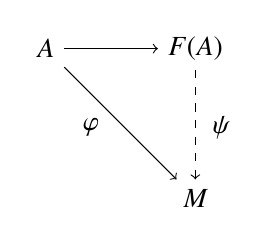
\begin{tikzpicture}[node distance=1.9cm]
          \node (A) {$A$};
          \node [right of=A] (free) {$F(A)$};
          \node [below of=free] (M) {$M$};
          \draw [->] (A) -- (free);
          \draw [->,dashed] (free) -- (M);
          \draw [->] (A) -- (M);
          \node [left] at (.8,-1) {$\phi$};
          \node [right] at (2, -1) {$\psi$};
     \end{tikzpicture}
 \end{center}
\vspace*{\stretch{1}}
\end{flashcard}

\begin{flashcard}[Modules]{True or False: If $F_1$ and $F_2$ are free $R$-modules on the same set $A$, then there is a unique isomorphism between $F_1$ and $F_2$ which is the identity map on $A$. Give a proof or counterexample.}
\vspace*{\stretch{1}}
 True.\\
 
 \emph{Proof sketch: }$F_1$ and $F_2$ are both a bunch of copies of $R$ indexed by the elements of $A$, so just map any copy of $R$ to another copy of $R$.
\vspace*{\stretch{1}}
\end{flashcard}

\begin{flashcard}[Modules]{Let $R$ be an integral domain and let $M$ be a free $R$-module of finite rank $n$. Prove that any $n+1$ elements of $M$ are $R$-linearly dependent.}
\vspace*{\stretch{1}}
 Let $x_1, \ldots, x_{n+1} \in M$ be our set of $n+1$ elements.\\
 
 $R$ is an integral domain, so embed it in its field of fractions $F$. Because $M \cong R^n$, we know $M \subseteq F^n$. Since $F^n$ is an $n$-dimensional vector space, the $n+1$ elements are $F$-linearly dependent so there exists linear dependence relation with $f_1, \ldots, f_{n+1} \in F$ not all zero such that $f_1 x_1 + \cdots f_{n+1} x_{n+1} = 0$. We can obtain an $R$-linear dependence relation by clearing the denominators.
\vspace*{\stretch{1}}
\end{flashcard}

\begin{flashcard}[Modules]{Let $R$ a ring and $M$ an $R$-module. What does it mean for $M$ to be a \underline{torsion module}?}
\vspace*{\stretch{1}}
 $M$ is a torsion module if for every $m \in M$, there exists $r \in R$ such that $r$ is not a zero divisor and $r$ annihilates $m$, i.e. $rm = 0$. In other words, every element of $M$ is a torsion element.
\vspace*{\stretch{1}}
\end{flashcard}

\begin{flashcard}[Modules]{Let $R$ a ring and $M$ an $R$-module. What does it mean for $M$ to be \underline{torsion-free}?}
\vspace*{\stretch{1}}
 $M$ is torsion free if for $m \in M$ and $r \in R$ where $r$ is not a zero divisor, $rm = 0$ implies that $m=0$. In other words, the only torsion element of $M$ is 0.
\vspace*{\stretch{1}}
\end{flashcard}

\begin{flashcard}[Modules]{Let $R$ an integral domain and $M$ an $R$-module. What is the \underline{torsion submodule} denoted $\Tor(M)$?}
\vspace*{\stretch{1}}
 The \emph{torsion submodule} $\Tor(M)$ is the set of all torsion elements of $M$. \\
 
 \emph{Note: }If $R$ is not commutative, $\Tor(M)$ may fail to be a submodule.
\vspace*{\stretch{1}}
\end{flashcard}

\begin{flashcard}[Modules]{Let $R$ be a ring, $M$ be an $R$-module, and $N$ a submodule of $M$. What is the \underline{annihilator} of $N$?}
\vspace*{\stretch{1}}
 The \emph{annihilator} of $N$ is the ideal of $R$ defined by
 $$
 \Ann(N) = \{r \in R \mid rn = 0 \text{ for all } n \in N \}
 $$
\vspace*{\stretch{1}}
\end{flashcard}

\begin{flashcard}[Modules]{True or False: If $M$ is an $R$-module for some ring $R$ and $N,L$ are submodules, then $N \subseteq L$ implies $\Ann{N} \subseteq \Ann{L}$.}
\vspace*{\stretch{1}}
 False. \\
 
 $\Ann(L) \subseteq \Ann(N)$
\vspace*{\stretch{1}}
\end{flashcard}

\begin{flashcard}[Modules]{Let $R$ be an integral domain. What is the \underline{rank} of an $R$-module $M$?}
\vspace*{\stretch{1}}
 The \emph{rank} of $M$ is the maximum number of $R$-linearly independent elements of $M$.
\vspace*{\stretch{1}}
\end{flashcard}

\begin{flashcard}[Modules]{True or False: Let $R$ be an integral domain, $M$ a finitely generated $R$-module, and $N$ a submodule of $M$. Then the rank of $M$ is greater than or equal to the rank of $N$.}
\vspace*{\stretch{1}}
 False. Consider $\Z[x]$ as a module over itself. Then its rank is one while the rank of its submodule $(2,x)$ is two. \\
 
 %(I can't find the source of this theorem and I'm not 100\% sure it's true.)
\vspace*{\stretch{1}}
\end{flashcard}

\begin{flashcard}[Modules]{State the structure theorem for modules over PIDs in invariant factor form.}
\vspace*{\stretch{1}}
 Let $R$ be a PID and $M$ a finitely generated $R$-module. Then
 \begin{enumerate}
      \item $M \cong R^n \oplus R/(a_1) \oplus R/(a_2) \oplus \cdots \oplus R/(a_m)$ where $a_i \in R$ nonzero and $a_1 \divides a_2 \divides \cdots \divides a_m.$
      \item $M$ is torsion-free if and only if $M$ is free.
      \item $\Tor(M) \cong R/(a_1) \oplus R/(a_2) \oplus \cdots \oplus R/(a_m)$
 \end{enumerate}
\vspace*{\stretch{1}}
\end{flashcard}

\begin{flashcard}[Modules]{State the structure theorem for modules over PIDs in elementary divisor form.}
\vspace*{\stretch{1}}
 Let $R$ be a PID and $M$ a finitely generated $R$-module. Then $M$ is the direct sum of a finite number of cyclic modules whose annihilators are either $(0)$ or generated by powers of primes in $R$, i.e.
 $$
 M \cong R^n \oplus R/(p_1^{\alpha_1}) \oplus R/(p_2^{\alpha_2}) \oplus \cdots \oplus R/(p_t^{\alpha_t})
 $$
 where $n$ is a nonnegative integer and $p_i^{\alpha_i}$ are positive powers of not-necessarily-distinct primes in $R$.
\vspace*{\stretch{1}}
\end{flashcard}

\begin{flashcard}[Modules]{Let $R$ be a PID and let $M$ be a \\torsion $R$-module, $M \neq 0$. \\What is the $p$-primary component of $M$?}
\vspace*{\stretch{1}}

$p_i$-primary component of $M$
$$=\{x\in M: xp_i^\alpha=0\text{ where }\alpha>0\}$$
% Suppose $a \in R$ annihilates $M$ and that $a$ factors into distinct prime powers in $R$ as $u p_1^{\alpha_1} \cdots p_n^{\alpha_n}$. The $p_i$-primary component of $M$ is $N_i = \{x \in M \mid p_i^{\alpha_i} = 0\}$. \\
 
% (There may be a mistake in this card that I can't find.)
\vspace*{\stretch{1}}
\end{flashcard}

\begin{flashcard}[Modules]{True or False: Every nonzero torsion module over a PID is a direct sum of its $p$-primary components. Give a proof or counterexample.}
\vspace*{\stretch{1}}
 True. \\
 
 Let $M$ be the aforementioned torsion module. By the structure theorem for modules over PIDs (elementary divisor form), the fact that $M$ is torsion means that its free rank is zero. Then the structure theorem states exactly this - that $M$ is isomorphic to a direct sum of its $p$-primary components.
\vspace*{\stretch{1}}
\end{flashcard}

\begin{flashcard}[Modules]{Let $R$ be a PID and $p$ prime in $R$. Let $F = R/(p)$. Prove that if $M = R^n$, then $M/pM \cong F^n$.}
\vspace*{\stretch{1}}
 We will proceed by seeking a $R$-module homomorphism $\phi: R^n \to (R/(p))^n$ with kernel $pM$.\\
 
 Take $(a_1, \ldots, a_n) \in R^n$ and let $\phi((a_1, \ldots, a_n)) = (a_1 \mod (p), \ldots, a_n \mod (p))$. This map is clearly surjective. The kernel is the set of elements whose every component are multiples of $p$, or in other words, $pR^n$. Thus $M / pM = R^n / p R^n \cong (R/(p))^n = F^n$.
\vspace*{\stretch{1}}
\end{flashcard}

\begin{flashcard}[Modules]{What is an \underline{$R$-algebra?}}
\vspace*{\stretch{1}}
 Let $R$ be a commutative ring. An \emph{$R$-algebra} is an $R$-module $M$ together with binary multiplication $M \times M \to M$ (called $M$-multiplication) satisfying
 \begin{itemize}
      \item $[\alpha x + \beta y, z] = \alpha[x,z] + \beta[y,z]$
      \item $[z, \alpha x + \beta y] = \alpha[z,x] + \beta[z,y]$
 \end{itemize}
for all scalars $\alpha, beta \in R$ and all elements $x,y,z \in A$.
\vspace*{\stretch{1}}
\end{flashcard}


\begin{flashcard}[Modules]{What is meant by the expression ``Every $R$-algebra is also an $R$-module''?}
\vspace*{\stretch{1}}
 Any $R$-algebra is an $R$-module by simply forgetting the multiplicative structure of that $R$-algebra.
\vspace*{\stretch{1}}
\end{flashcard}

\begin{flashcard}[Modules]{What is special about a module over a PID?}
\vspace*{\stretch{1}}
 A module over a PID has a decomposition based on the Structure Theorem for Modules over PIDs.
\vspace*{\stretch{1}}
\end{flashcard}


\begin{flashcard}[Modules]{True or False: Let $F$ be a field. Any nonzero free $F[x]$-module is an infinite dimensional vector space over $F$. Give a proof or counterexample.}
\vspace*{\stretch{1}}
 True. \\
 
 Since $F$ is a field, $F[x]$ is a PID. By the Structure Theorem for Modules over PIDs, a free $F[x]$-module is isomorphic to a direct sum of copies of $F[x]$.
\vspace*{\stretch{1}}
\end{flashcard}
% 
% \begin{flashcard}[Modules]{front}
% \vspace*{\stretch{1}}
%  back
% \vspace*{\stretch{1}}
% \end{flashcard}
% 
% \begin{flashcard}[Modules]{front}
% \vspace*{\stretch{1}}
%  back
% \vspace*{\stretch{1}}
% \end{flashcard}
% 
% \begin{flashcard}[Modules]{front}
% \vspace*{\stretch{1}}
%  back
% \vspace*{\stretch{1}}
% \end{flashcard}
% 
% \begin{flashcard}[Modules]{front}
% \vspace*{\stretch{1}}
%  back
% \vspace*{\stretch{1}}
% \end{flashcard}
% 
% \begin{flashcard}[Modules]{front}
% \vspace*{\stretch{1}}
%  back
% \vspace*{\stretch{1}}
% \end{flashcard}
% 
% \begin{flashcard}[Modules]{front}
% \vspace*{\stretch{1}}
%  back
% \vspace*{\stretch{1}}
% \end{flashcard}
% 
% \begin{flashcard}[Modules]{front}
% \vspace*{\stretch{1}}
%  back
% \vspace*{\stretch{1}}
% \end{flashcard}
% 
% \begin{flashcard}[Modules]{front}
% \vspace*{\stretch{1}}
%  back
% \vspace*{\stretch{1}}
% \end{flashcard}
% 
% \begin{flashcard}[Modules]{front}
% \vspace*{\stretch{1}}
%  back
% \vspace*{\stretch{1}}
% \end{flashcard}
% 
% \begin{flashcard}[Modules]{front}
% \vspace*{\stretch{1}}
%  back
% \vspace*{\stretch{1}}
% \end{flashcard}
% 
% \begin{flashcard}[Modules]{front}
% \vspace*{\stretch{1}}
%  back
% \vspace*{\stretch{1}}
% \end{flashcard}
% 
% \begin{flashcard}[Modules]{front}
% \vspace*{\stretch{1}}
%  back
% \vspace*{\stretch{1}}
% \end{flashcard}
% 
% \begin{flashcard}[Modules]{front}
% \vspace*{\stretch{1}}
%  back
% \vspace*{\stretch{1}}
% \end{flashcard}
% 
% \begin{flashcard}[Modules]{front}
% \vspace*{\stretch{1}}
%  back
% \vspace*{\stretch{1}}
% \end{flashcard}







%%%%% This section uses Roman's Advanced Linear Algebra Chapter 4%%%%%

\begin{flashcard}[Modules]{True or False: Let $R$ be a ring and $M$ an $R$-module. if $A$ is a minimal spanning set for $M$ under $R$-linear combinations, then $A$ is a basis. Give a proof or counterexample.}
\vspace*{\stretch{1}}
 False. \\
 
 Let $\Z/n\Z$ be a $\Z$-module. This module cannot have a basis because no element is linearly independent, i.e. every element can be multiplied by an appropriate nonzero element of $\Z$ to reach 0. So $1 \in \Z/n\Z$ is a minimal spanning set, yet it fails to be a basis.
\vspace*{\stretch{1}}
\end{flashcard}

\begin{flashcard}[Modules]{True or False: Let $R$ be a ring and $M$ an $R$-module with a finite basis. Then every spanning set in $M$ contains a basis and every linearly independent set in $M$ is contained in a basis.}
\vspace*{\stretch{1}}
 False. \\
\vspace*{\stretch{1}}
\end{flashcard}

\begin{flashcard}[Modules]{Give an example of a free module with a submodule that is not free.}
\vspace*{\stretch{1}}
 The set $\Z \times \Z$ is a free module over itself using componentwise multiplication. We know it is free because the singleton set $\{(1,1)\}$ serves as a basis.\\
 
 The submodule $\Z \times \{0\}$ is a proper submodule that is not free. We know it is not free because no elements are linearly independent. Any $(a,0)$ is torsion because multiplying by nonzero element $(0,b)$ will result in $(0,0)$.
\vspace*{\stretch{1}}
\end{flashcard}

\begin{flashcard}[Modules]{True or False: If $M$ is an $R$-module for some ring $R$, then $M$ is a free $R$-module if and only if $M$ has a basis.}
\vspace*{\stretch{1}}
 True.
\vspace*{\stretch{1}}
\end{flashcard}

\begin{flashcard}[Modules]{For what kind of $R$-module is is true that we can uniquely define an $R$-module homomorphism by specifying the values that the elements of a basis map to?}
\vspace*{\stretch{1}}
 This is true for free $R$-modules. \\
 
 Only free $R$-modules have bases anyway!
\vspace*{\stretch{1}}
\end{flashcard}

\begin{flashcard}[Modules]{Give an example of a quotient of a free module that is not free.}
\vspace*{\stretch{1}}
 $\Z$ is a free module over itself because its basis is the set $\{1\}$. $n\Z$ is is a proper submodule that is also free because its basis is the set $\{n\}$. But $\Z/n\Z$ is not a free $\Z$-module because not even a single element is linearly independent.
\vspace*{\stretch{1}}
\end{flashcard}

\begin{flashcard}[Modules]{Give an example of an $R$-module that cannot be expressed as a direct sum of it submodules.}
\vspace*{\stretch{1}}
 $\Z$ is a module over itself. Its submodules are the ideals of the ring $\Z$. These are $n\Z$ for $n \in Z$.\\
 
 Given any two submodules $n\Z$ and $m\Z$, we know that their intersection is nontrivial. In fact, their interseciton is $k\Z$ where $k = \lcm(n,m).$ Since there are no submodules that intersect only trivially, this module cannot be expressed as a direct sum.
\vspace*{\stretch{1}}
\end{flashcard}

\begin{flashcard}[Modules]{Let $M$ be an $R$-module for some ring $R$ and let $N,P$ be submodules. Prove that if $M = N \oplus P$, then $P \cong M/N.$}
\vspace*{\stretch{1}}
 Let $\pi$ be the canonical projection $\pi: M \to P$. Then by the first isomorphism theorem, $M/N \cong P$.
\vspace*{\stretch{1}}
\end{flashcard}

\begin{flashcard}[Modules]{Let $M$ an $R$-module for some ring $R$. What condition needs to be placed on $R$ to guarantee that any two bases of $M$ have the same cardinality and the cardinality of a spanning set is greater than or equal to that of a basis?}
\vspace*{\stretch{1}}
 $R$ needs to be a commutative ring with identity.
\vspace*{\stretch{1}}
\end{flashcard}

\begin{flashcard}[Modules]{Complete the sentence: Let $R$ be a commutative ring with identity. Then two $R$-modules have the same rank if and only if \blank.}
\vspace*{\stretch{1}}
 they are isomorphic
\vspace*{\stretch{1}}
\end{flashcard}

\begin{flashcard}[Modules]{Let $R$ be  PID and let $M$ be a cyclic $R$-module. Let $\Ann(M)$ be the annihilator of $M$. Prove that $M \cong R/Ann(M)$.}
\vspace*{\stretch{1}}
 Define the multiplication map $\phi$ such that for $r \in R$, $m \in M$, $\phi(r) = rm$. This is an $R$-module homomorphism. The map is surjective since $M$ is cyclic. The kernel of this map is the set of elements in $R$ that map every element of $M$ to zero - in other words, $\Ann(M)$. Thus by the first isomorphism theorem, $R/\Ann(M) \cong M.$
\vspace*{\stretch{1}}
\end{flashcard}

\begin{flashcard}[Modules]{What condition on a ring $R$ guarantees that any submodule of a free $R$-module is also free?}
\vspace*{\stretch{1}}
 $R$ is a PID.
\vspace*{\stretch{1}}
\end{flashcard}

\begin{flashcard}[Modules]{True or False: Let $M$ be a free module over $R$ and let $R$ be a PID. Let $N$ be a submodule of $M$. Then any basis for $N$ can be extended to form a basis for $M$. Give a proof or counterexample.}
\vspace*{\stretch{1}}
 False. \\
 
 $\Z$ is a module over itself and $2\Z$ is a submodule. The set $\{2\}$ is a basis for $2\Z$, but it cannot be extended to a basis for $\Z$.
\vspace*{\stretch{1}}
\end{flashcard}

\begin{flashcard}[Modules]{Let $R$ be a PID, $M$ a free $R$-module, and $N$ a submodule. What is the closest analogue to the vector space property that there is a basis for $M$ containing a basis for $N$?}
\vspace*{\stretch{1}}
 Let $M$ be of rank $n$ and let $N$ be of rank $k \leq n$. Then there is a basis $\mathcal{B}$ for $M$ that contains a subset $S = \{v_1, \ldots, v_k\}$ for which $\{r_1v_1, \ldots, r_kv_k \}$, $r_i \in R$ nonzero, is a basis for $N$. The elements $r_i$ satisfy the divisility relations $r_1 \divides r_2 \divides \cdots \divides r_k$
\vspace*{\stretch{1}}
\end{flashcard}

\begin{flashcard}[Modules]{True or False: Any free module over an integral domain is torsion-free. Give a proof or counterexample.}
\vspace*{\stretch{1}}
 True. \\
 
 A free module of rank $n$ over $R$ where $R$ is an integral domain is isomorphic to $R^n$. Since $R$ is an integral domain, its action on $R^n$ ($n$ copies of itself) must be torsion-free.
\vspace*{\stretch{1}}
\end{flashcard}

\begin{flashcard}[Modules]{Complete the sentence: A finitely-generated module over a PID is a free module if and only if it is \blank.}
\vspace*{\stretch{1}}
 torsion-free
\vspace*{\stretch{1}}
\end{flashcard}

\begin{flashcard}[Modules]{Complete the sentence: Any \blank module over a PID $R$ is the direct sum of a finitely generated free $R$-module and a finitely generated torsion $R$-module}
\vspace*{\stretch{1}}
 finitely generated\\
\vspace*{\stretch{1}}
\end{flashcard}

\begin{flashcard}[Modules]{Let $R$ be a PID and $M$ a finitely generated $R$-module so that $M \cong M_\text{free} \oplus M_\text{tor}$. \\True or False: \\(1) $M_\text{free}$ is unique. \\(2) $M_\text{tor}$ is unique.}
\vspace*{\stretch{1}}
\begin{enumerate}
     \item False. $M_\text{free}$ is unique up to isomorphism, i.e., its rank is unique
     \item True. $M_\text{tor}$ consists of all the torsion elements of $M$.
\end{enumerate}
\vspace*{\stretch{1}}
\end{flashcard}

%%%%% End of section using Roman's book %%%%%



%%%% LINEAR ALGEBRA %%%%% 

\begin{flashcard}[Linear Algebra]{When does a matrix admit an $LU$ decomposition into lower and upper triangular matrices?}
\vspace*{\stretch{1}}
 An invertible matrix admits an $LU$ decomposition if and only if all of its leading principal minors are nonsingular, i.e. all of the $(n-1) \times (n-1)$ minors are nonsingular.
\vspace*{\stretch{1}}
\end{flashcard}

\begin{flashcard}[Linear Algebra]{What are the vector space axioms for a vector space $V$ over a field $F$?}
\vspace*{\stretch{1}}
 For $u,v \in V$ and $a,b \in F$, we must have
  \begin{enumerate}
   \item $V$ is a group under addition
   \item $a(bv) = (ab)v$
   \item $1v = v$ where $1 \in F$
   \item a(u+v) = au + av
   \item (a+b)v = av + bv
  \end{enumerate}
\vspace*{\stretch{1}}
\end{flashcard}

\begin{flashcard}[Linear Algebra]{Fill in the blank: Each conjugacy class of \blank is represented by exactly one matrix in rational canonical form}
\vspace*{\stretch{1}}
 $GL_n(F)$ for some field $F$. This means that you can use RCF to count conjugacy classes in $GL_n(F)$ but not in some subgroup, say $SL_n(F).$
\vspace*{\stretch{1}}
\end{flashcard}

\begin{flashcard}[Linear Algebra]{Given a matrix $A$, what is the \underline{trace} of $A$? What are the three properties that completely characterize a matrix trace?}
\vspace*{\stretch{1}}
 The trace of $A$ is the sum along its diagonal. The three properties that completely characterize the trace are
 \begin{enumerate}
      \item $\tr(A+B) = \tr(A) + \tr(B)$
      \item $\tr(cA) = c\tr(A)$ for constant $c$
      \item $\tr(AB) = \tr(BA)$
 \end{enumerate}

\vspace*{\stretch{1}}
\end{flashcard}

\begin{flashcard}[Linear Algebra]{True or False: Given a finite collection of matrices, the trace of their product is the same for any order matrix multiplication.}
\vspace*{\stretch{1}}
 False.\\
 
 The trace is only equal for \emph{cyclic} permutations of the order of multiplication. Thus $\tr(ABC) = \tr(BCA) = \tr(CAB)$ but $\tr(ABC) \neq \tr(ACB)$
\vspace*{\stretch{1}}
\end{flashcard}

\begin{flashcard}[Linear Algebra]{Let $V$ be a vector space over field $F$ and $S$ a subset of $V$. What does it mean for $S$ to be a \underline{linearly independent} set of vectors?}
\vspace*{\stretch{1}}
 $S$ is a \emph{linearly independent} set of vectors if for $\alpha_1, \ldots, \alpha_n \in F$ and $v_1, \ldots, v_n \in S$, the equation $\alpha_1 v_1 + \cdots + \alpha_n v_n = 0$ implies that $\alpha_1 = \cdots = \alpha_n = 0$.
\vspace*{\stretch{1}}
\end{flashcard}

\begin{flashcard}[Linear Algebra]{Let $V$ be a vector space. What is a \underline{basis} for $V$?}
\vspace*{\stretch{1}}
 A \emph{basis} for $V$ is a minimal spanning set. It can also be described as a maximal linearly independent set.
\vspace*{\stretch{1}}
\end{flashcard}

\begin{flashcard}[Linear Algebra]{Let $V,W$ be two $n$-dimensional vector spaces over a field $F$. Prove that $V$ and $W$ are isomorphic.}
\vspace*{\stretch{1}}
 We will prove that $V$ and $W$ are both isomorphic to $F^n$. Let $v_1, \ldots, v_n$ be a basis for $V$. Define the map 
 $$\phi: F^n \to V \qquad by \qquad \phi(\alpha_1, \ldots, \alpha_n) = \alpha_1 v_1 + \cdots + \alpha_n v_n$$
 
 It is clear that $\phi$ is $F$-linear, surjective, and injective. Thus $\phi$ is an isomorphism.
\vspace*{\stretch{1}}
\end{flashcard}

\begin{flashcard}[Linear Algebra]{Let $V$ be a vector space over $F$ and $W$ a subspace of $V$. What is the dimension of $V/W$?}
\vspace*{\stretch{1}}
 $\dim V/W = \dim V - \dim W$
\vspace*{\stretch{1}}
\end{flashcard}

\begin{flashcard}[Linear Algebra]{Let $\phi: V \to U$ be a linear transformation over $F$. What is the relationship between $\dim V$, $\dim \ker \phi$, and $\dim \phi(V)$?}
\vspace*{\stretch{1}}
 $\dim V = \dim \ker \phi + \dim \phi(V)$
\vspace*{\stretch{1}}
\end{flashcard}

\begin{flashcard}[Linear Algebra]{Let $V$ be a $k$-dimensional vector space over $F_q$, the finite field with $q$ elements. How many distinct bases of $W$ are there? How does this relate to $|GL(V)|$, the group of invertible linear transformations from $V$ to $V$?}
\vspace*{\stretch{1}}
 There are $(q^k - 1)(q^k - q)(q^k - q^2)\cdots(q^k - q^{k-1})$ distinct bases of $V$. The first basis vector is one of the $q^k - 1$ nonzero vectors. The second one is a vector not in the span of the first, so there are $q^k - q$ possibilities. The third is not in the span of the first two vectors, so there are $q^k - q^2$ possibilities. We continue this way until we have $k$ vectors.\\
 
 $|GL(V)|$ is equal to this same number because an invertible map from $V$ maps a fixed basis to any basis of $V$, so there are exactly as many as distinct bases for $V$.
\vspace*{\stretch{1}}
\end{flashcard}

\begin{flashcard}[Linear Algebra]{Suppose $\phi: \Q^3 \to \Q^3$ is a linear transformation such for $x,y,z \in \Q$, $\phi(x,y,z) = (9x+4y+5z, -4x-3z, -6x-4y-2z)$. Write the matrix representing $\phi$.}
\vspace*{\stretch{1}}
 \emph{Erica says: } Rows describe where you go. Columns describe where you're fro $\ldots$ lum.
 $$
 \left ( \begin{array}{ccc}
      9 & 4 & 5 \\
      -4 & 0 & -3 \\
      -6 & -4 & -2
 \end{array} \right )
$$
Note that the first row is the coefficient of $x$, i.e. it's where x ``goes''. The first column lists the coefficients of $x,y,z$, thereby describing where the image is ``frolum.''
\vspace*{\stretch{1}}
\end{flashcard}

\begin{flashcard}[Linear Algebra]{Let $V,W$ be vector spaces over field $F$. What is the dimension of $\Hom_F(V,W)$? Give a proof.}
\vspace*{\stretch{1}}
 $\dim \Hom_F(V,W) = (\dim V)(\dim W)$\\
 
 \emph{Pf: }$\Hom_F(V,W)$ is isomorphic to the space of $(\dim V) \times (\dim W)$ matrices over $F$. The space of these matrices has dimension $(\dim V)(\dim W)$.
\vspace*{\stretch{1}}
\end{flashcard}

\begin{flashcard}[Linear Algebra]{Let $A,B$ be $n \times n$ matrices. What does it mean if $A$ and $B$ are \underline{similar}?}
\vspace*{\stretch{1}}
 $A$ and $B$ are \emph{similar} if there exists an invertible $n \times n$ matrix $P$ such that $A = P \inv B P$.\\
 
 Geometrically, this means they represent the same linear transformation under a difference choice of basis.
\vspace*{\stretch{1}}
\end{flashcard}

\begin{flashcard}[Linear Algebra]{Let $V$ be a vector space over field $F$. What is the \underline{dual space} $V^*$?}
\vspace*{\stretch{1}}
 \emph{Cherry says: } the lying down vectors!\\
 
 $V^* = \Hom_F(V,F)$, i.e. the space of linear transformations from $V$ to $F$.\\
 
 The elements of $V^*$ are called \emph{linear functionals}.
\vspace*{\stretch{1}}
\end{flashcard}

\begin{flashcard}[Linear Algebra]{Let $V$ be a vector space over field $F$. Given some basis $\{v_1, \ldots, v_n \}$ of $V$, what is the \underline{dual basis}?}
\vspace*{\stretch{1}}
 The \emph{dual basis} is the set $\{v_1^*, \ldots, v_n^*\}$ such that the action of any element of the dual basis on any element of the basis of $V$ is defined by $v_i^*(v_j) = \delta_{ij}$, i.e. the Kronecker delta.\\
 
 As the name suggests, the dual basis is a basis for dual space $V^*$.
\vspace*{\stretch{1}}
\end{flashcard}

\begin{flashcard}[Linear Algebra]{True or False: Let $V$ be a vector space and $V^*$ its dual space. Then $\dim(V) = \dim(V^*)$.}
\vspace*{\stretch{1}}
 False. \\
 
 If $V$ is finite dimensional, the statement is true since $\dim V^* = \dim \Hom_F(V,F) = (\dim V)(\dim F) = \dim V$. \\
 
If $V$ is infinite dimensional, $\dim(V) < \dim(V^*)$.
\vspace*{\stretch{1}}
\end{flashcard}

\begin{flashcard}[Linear Algebra]{Let $V$ be a vector space over field $F$. What is the \underline{double dual} $V^{**}$?}
\vspace*{\stretch{1}}
 It is the dual of $V^*$.
\vspace*{\stretch{1}}
\end{flashcard}

\begin{flashcard}[Linear Algebra]{Let $V$ be a finite-dimensional vector space. What does it mean to say that there is a natural isomorphism between $V$ and its double dual $V^{**}$? What is this isomorphism?}
\vspace*{\stretch{1}}
 It means that specifying an explicit isomorphism between the two spaces does not depend on choosing a basis.\\
 
 This isomorphism is called \emph{evaluation at $v$}. Define
 $$
 E_v: V^* \to F \qquad \text{by} \qquad E_v(f) = f(v).
 $$
 Then $\phi: V \to V^{**}$ such that $\phi(v) = E_v$ is an isomorphism.
\vspace*{\stretch{1}}
\end{flashcard}

% I skipped all the stuff on alternating multilinear forms and went straight to the defn of determinant. Is that okay?

\begin{flashcard}[Linear Algebra]{Given a matrix $A = (\alpha_{ij})$, what is the \underline{determinant}?}
\vspace*{\stretch{1}}
 The determinant, denoted $\det(A)$, is given by
 $$
 \det(\alpha_{ij}) = \sum_{\sigma \in S_n} \sgn(\sigma) \prod_{i=1}^n \alpha_{\sigma(i)i}
 $$
 where $\sgn(\sigma)$ is the sign (+ or -) of the permutation $\sigma$.
\vspace*{\stretch{1}}
\end{flashcard}

\begin{flashcard}[Linear Algebra]{State \underline{Cramer's Rule}.}
\vspace*{\stretch{1}}
 Let $A_1, \ldots, A_n$ be the columns of $n \times n$ matrix $A$. Suppose $B = \beta_1 A_1 + \cdots \beta_n A_n$ for $\beta_1, \ldots, \beta_n \in R$, $R$ a ring. Then
 $$
 \beta_i \det A = \det(A_1, \ldots, A_{i-1}, B, A_{i+1}, \ldots, A_n)
 $$
\vspace*{\stretch{1}}
\end{flashcard}

\begin{flashcard}[Linear Algebra]{Let $A$ be an $n \times n$ matrix over an integral domain $R$. What can we say about the columns of $A$ if $\det A = 0$?}
\vspace*{\stretch{1}}
 $\det A = 0$ if and only if the columns of $A$ are $R$-linearly dependent.
\vspace*{\stretch{1}}
\end{flashcard}

\begin{flashcard}[Linear Algebra]{True or False: Let $A,B$ be $n \times n$ matrices over a commutative unital ring $R$. Then $\det AB = (\det A) (\det B)$.}
\vspace*{\stretch{1}}
 True.
\vspace*{\stretch{1}}
\end{flashcard}

\begin{flashcard}[Linear Algebra]{True or False: If $W$ is any subspace of vector space $V$, then there exists subspace $U$ such that $V = W \oplus U$. Give a proof or a counterexample.}
\vspace*{\stretch{1}}
 True. Every subspace has a complement. \\
 
 Let $B_W$ be a basis for $W$. We can extend it to form a basis for $V$. Let this basis for $V$ be called $B_V$. Then $U$ is the span of $B_V \setminus B_W.$ By the construction of $B_V$, it is clear that $V = W \oplus U$. 
\vspace*{\stretch{1}}
\end{flashcard}

\begin{flashcard}[Linear Algebra]{Let $T$ be the matrix of a linear transformation. How does one calculate $\det(T)$ if $T$ is upper triangular?}
\vspace*{\stretch{1}}
 $\det(T) = \text{ the product along the diagonal}$
\vspace*{\stretch{1}}
\end{flashcard}

\begin{flashcard}[Linear Algebra]{Let $T$ be the matrix of a linear transformation. How does one find the characteristic polynomial of $T$?}
\vspace*{\stretch{1}}
 The characteristic polynomial is $\det(xI - T)$.
\vspace*{\stretch{1}}
\end{flashcard}

\begin{flashcard}[Linear Algebra]{What is the significance of the roots of the characteristic polynomial?}
\vspace*{\stretch{1}}
 They are eigenvalues.
\vspace*{\stretch{1}}
\end{flashcard}

\begin{flashcard}[Linear Algebra]{What is the \underline{minimal polynomial} of a matrix $A$?}
\vspace*{\stretch{1}}
 The \emph{minimal polynomial} $m(x)$ is the unique monic polynomial of lowest degree such that $m(A) = 0$ (the zero operator)
\vspace*{\stretch{1}}
\end{flashcard}

\begin{flashcard}[Linear Algebra]{Explain the fact that the rational canonical form of a matrix $A$ is based on an invariant factor decomposition of the finite-dimensional vector space $V$.}
\vspace*{\stretch{1}}
 Given a particular matrix $A$, $V$ is an $F[x]$-module. Since $F[x]$ is a PID (actually it's Euclidean), we can use the structure theorem for modules over PIDs. Then 
 $$ V \cong F[x]/(a_1(x)) \oplus F[x]/(a_2(x)) \oplus \cdots \oplus F[x]/(a_m(x))$$
 
 where the generators of the quotienting ideals are invariant factors.
\vspace*{\stretch{1}}
\end{flashcard}

\begin{flashcard}[Linear Algebra]{True or False: The minimal polynomial is the smallest invariant factor of vector space $V$.}
\vspace*{\stretch{1}}
 False.\\
 
 It is the largest invariant factor. All other invariant factors must divide it.
\vspace*{\stretch{1}}
\end{flashcard}

\begin{flashcard}[Linear Algebra]{Given an invariant factor $a(x) = x^n + b_{n-1}x^{n-1} + \cdots + b_1 x + b_0$, what is the companion matrix generated by this invariant factor?}
\vspace*{\stretch{1}}
 $$ \left ( 
 \begin{array}{cccccc}
      0 & 0 & \cdots & \cdots & \cdots & -b_0 \\
      1 & 0 & \cdots & \cdots & \cdots & -b_1 \\
      0 & 1 & \cdots & \cdots & \cdots & -b_2 \\
      0 & 0 & \ddots &&& \vdots \\
      \vdots & \vdots &&\ddots&& \vdots \\
      0 & 0 & \cdots & \cdots & 1 & -b_{n-1} \\
 \end{array}
 \right)$$
\vspace*{\stretch{1}}
\end{flashcard}

\begin{flashcard}[Linear Algebra]{Let $\mathcal{C}_i$ be the companion matrix calculated from invariant factor $a_i(x)$ and let the invariant factors satify $a_1(x) \divides a_2(x) \divides \cdots \divides a_m(x)$. How do we form the rational canonical form from these companion matrices? }
\vspace*{\stretch{1}}
 $$ \left ( 
 \begin{array}{cccc}
      \mathcal{C}_1 &&& \\
      & \mathcal{C}_2 && \\
      && \ddots & \\
      &&& \mathcal{C}_m
 \end{array}
 \right)$$
\vspace*{\stretch{1}}
\end{flashcard}

\begin{flashcard}[Linear Algebra]{True or False: Let $S,T$ be linear transformations of $V$. Then $S,T$ are similar if and only if they share the same rational canonical form.}
\vspace*{\stretch{1}}
 True.
\vspace*{\stretch{1}}
\end{flashcard}

\begin{flashcard}[Linear Algebra]{True or False: Let $A$ be an $n \times n$ matrix over field $F$ and let $K$ be an extension of $F$. Then the rational canonical forms of $A$ over $K$ and over $F$ are the same. }
\vspace*{\stretch{1}}
 True.
\vspace*{\stretch{1}}
\end{flashcard}

\begin{flashcard}[Linear Algebra]{What is an \underline{$n \times n$ Jordan block for eigenvalue $\lambda$?}}
\vspace*{\stretch{1}}
 $$
 \left (
 \begin{array}{ccccc}
      \lambda & 1 &&& \\
      & \lambda & \ddots && \\
      && \ddots & 1 & \\
      &&& \lambda & 1 \\
      &&&& \lambda
 \end{array}
 \right )
 $$
\vspace*{\stretch{1}}
\end{flashcard}

\begin{flashcard}[Linear Algebra]{Complete the sentence: A matrix is diagonalizable if and only if its Jordan canonical form is \blank .}
\vspace*{\stretch{1}}
 diagonal
\vspace*{\stretch{1}}
\end{flashcard}

\begin{flashcard}[Linear Algebra]{In what sense is the Jordan canonical form of a matrix unique?}
\vspace*{\stretch{1}}
 It is unique up to permutation of the Jordan blocks.
\vspace*{\stretch{1}}
\end{flashcard}

\begin{flashcard}[Linear Algebra]{What does it mean for a matrix to be in \underline{Jordan canonical form}?}
\vspace*{\stretch{1}}
 A matrix is in \emph{Jordan canonical form} if it is block diagonal and each block is a Jordan block.
\vspace*{\stretch{1}}
\end{flashcard}

\begin{flashcard}[Linear Algebra]{True or False: Two diagonal matrices are similar if and only if their diagonal entries are the same up to a permutation.}
\vspace*{\stretch{1}}
 True. \\
 
 If their diagonal entries are the same up to permutation, then their Jordan canonical forms are the same, which means they are similar.
\vspace*{\stretch{1}}
\end{flashcard}

\begin{flashcard}[Linear Algebra]{A matrix $M$ is diagonalizable if and only if what condition is placed on its minimal polynomial? Give a proof.}
\vspace*{\stretch{1}}
 Its minimal polynomial $m(x)$ must have no repeated roots.\\
 
 $(\Longleftarrow)$ If $m(x)$ has no repeated roots, by the divisibility conditions of invariant factors, the elementary divisors are linear polynomials. Thus the JCF of $M$ is diagonal\\
 
 $(\Longrightarrow)$ If $M$ is similar to a diagonal matrix $D$, then $M$ and $D$ have the same minimal polynomial. The minimal polynomial of $D$ must contain all distinct linear factors, each corresponding to the $1 \times 1$ blocks that make up $D$.
\vspace*{\stretch{1}}
\end{flashcard}

% \begin{flashcard}[Linear Algebra]{front}
% \vspace*{\stretch{1}}
%  back
% \vspace*{\stretch{1}}
% \end{flashcard}
% 
% \begin{flashcard}[Linear Algebra]{front}
% \vspace*{\stretch{1}}
%  back
% \vspace*{\stretch{1}}
% \end{flashcard}
% 
% \begin{flashcard}[Linear Algebra]{front}
% \vspace*{\stretch{1}}
%  back
% \vspace*{\stretch{1}}
% \end{flashcard}
% 
% \begin{flashcard}[Linear Algebra]{front}
% \vspace*{\stretch{1}}
%  back
% \vspace*{\stretch{1}}
% \end{flashcard}
% 
% \begin{flashcard}[Linear Algebra]{front}
% \vspace*{\stretch{1}}
%  back
% \vspace*{\stretch{1}}
% \end{flashcard}
% 
% \begin{flashcard}[Linear Algebra]{front}
% \vspace*{\stretch{1}}
%  back
% \vspace*{\stretch{1}}
% \end{flashcard}
% 
% \begin{flashcard}[Linear Algebra]{front}
% \vspace*{\stretch{1}}
%  back
% \vspace*{\stretch{1}}
% \end{flashcard}
% 
% \begin{flashcard}[Linear Algebra]{front}
% \vspace*{\stretch{1}}
%  back
% \vspace*{\stretch{1}}
% \end{flashcard}
% 
% \begin{flashcard}[Linear Algebra]{front}
% \vspace*{\stretch{1}}
%  back
% \vspace*{\stretch{1}}
% \end{flashcard}
% 
% \begin{flashcard}[Linear Algebra]{front}
% \vspace*{\stretch{1}}
%  back
% \vspace*{\stretch{1}}
% \end{flashcard}
% 
% \begin{flashcard}[Linear Algebra]{front}
% \vspace*{\stretch{1}}
%  back
% \vspace*{\stretch{1}}
% \end{flashcard}
% 
% \begin{flashcard}[Linear Algebra]{front}
% \vspace*{\stretch{1}}
%  back
% \vspace*{\stretch{1}}
% \end{flashcard}




 






%%%% FIELDS %%%%

\begin{flashcard}[Fields]{In what fields does that quadratic formula apply?}
\vspace*{\stretch{1}}
 The quadratic formula applies in any field that is not of characteristic 2.
\vspace*{\stretch{1}}
\end{flashcard}

\begin{flashcard}[Fields]{Let $L/F$ be a finite extension of fields. For $\alpha \in L$, left multiplication by $\alpha$ is an $F$-linear transformation of $F$. What is the relationship between the field norm of $\alpha$ and this linear transformation induced by $\alpha$?}
\vspace*{\stretch{1}}
 Let $T$ be the matrix that represents the linear transformation. Then the field norm of $\alpha$ is the determinant of $T$.
\vspace*{\stretch{1}}
\end{flashcard}

\begin{flashcard}[Fields]{Let $L/F$ be a finite extension of fields. For $\alpha \in L$, what is the field norm $N_{L/F}(\alpha)$?}
\vspace*{\stretch{1}}
 Let $f(x)$ be the minimal polynomial for $\alpha$ over $F$. Let $\sigma_1(\alpha), \ldots, \sigma_n(\alpha)$ be the roots (counted with multiplicity) of $f(x)$. Then
 $$
 N_{L/F}(\alpha) = \left ( \prod_{j=1}^n \sigma_j(\alpha) \right) ^{[L:F(\alpha)]}
 $$
 i.e., it is the product of all Galois conjugates of $\alpha$. One can also think of it as the constant term of the minimal polynomial times $(-1)^n$ where $n$ is the degree of $f(x)$.
\vspace*{\stretch{1}}
\end{flashcard}

\begin{flashcard}[Fields]{Let $K/F$ be a finite extension of fields. For $\alpha \in K$, left multiplication by $\alpha$ on $K$ is an $F$-linear transformation $T_\alpha$ of $K$. How does the minimal polynomial of $\alpha$ over $F$ relate to $T_\alpha$?}
\vspace*{\stretch{1}}
 The minimal polynomial of $\alpha$ over $F$ is equal to the minimal polynomial of the matrix $T_\alpha$.
\vspace*{\stretch{1}}
\end{flashcard}

\begin{flashcard}[Fields]{Let $K/F$ be a finite extension of fields. For $\alpha \in K$, left multiplication by $\alpha$ on $K$ is an $F$-linear transformation $T_\alpha$ of $K$. What is the trace $Tr_{K/F}(\alpha)$? How does $Tr_{K/F}(\alpha)$ relate to $T_\alpha$?}
\vspace*{\stretch{1}}
  Let $f(x)$ be the minimal polynomial for $\alpha$ over $F$. Let $\sigma_1(\alpha), \ldots, \sigma_n(\alpha)$ be the roots (counted with multiplicity) of $f(x)$. Then
 $$
 Tr_{K/F}(\alpha) = \left ( \sum_{j=1}^n \sigma_j(\alpha) \right) ^{[L:F(\alpha)]}
 $$
 i.e., it is the sum of all Galois conjugates of $\alpha$. One can also think of it as the coefficient of the second-highest degree term of $f(x)$ times $-1$.
\vspace*{\stretch{1}}
\end{flashcard}

\begin{flashcard}[Fields]{Let $K/F$ be a finite extension of fields. For $\alpha \in K$, left multiplication by $\alpha$ is an $F$-linear transformation of $F$. What is the relationship between $Tr_{K/F}(\alpha)$ and this linear transformation induced by $\alpha$?}
\vspace*{\stretch{1}}
 $Tr_{K/F}(\alpha)$ is equal to the trace (matrix trace, i.e. sum along diagonal) of the matrix that represents the linear transformation.
\vspace*{\stretch{1}}
\end{flashcard}

\begin{flashcard}[Fields]{Let $F_{p^n}$ and $F_{p^m}$ be finite fields of characteristic $p$. What is the smallest finite field that contains both of them? Give a proof.}
\vspace*{\stretch{1}}
 Let $k = \lcm(n,m)$. Then the smallest finite field that contains both fields if $F_{p^k}$.\\
 
 $F_n$ contains the $n$ roots of $x^{p^n} - x$ and $F_m$ contains the $m$ roots of $x^{p^m} - x$. The smallest polynomial of the form $x^{p^k} - x$ that is divisible by both $x^{p^n} - x$ and $x^{p^m} - x$ is the one where $k = \lcm(n,m)$. Thus the smallest field that contains both fields is $F_{p^k}.$
\vspace*{\stretch{1}}
\end{flashcard}

\begin{flashcard}[Fields]{For what type of polynomial is is true that the polynomial is irreducible if and only if it does not have a root in field $F$?}
\vspace*{\stretch{1}}
 A polynomial of degree 2 or 3, since these are the only kinds that factor if and only if they have a linear factor.
\vspace*{\stretch{1}}
\end{flashcard}

\begin{flashcard}[Fields]{State the rational roots theorem}
\vspace*{\stretch{1}}
 Let $p(x)$ be a polynomial with integer coefficients. For $r/s \in \Q$, $r/s$ is a root of $p(x)$ if and only if $r$ divides the constant term  and $s$ divides the leading coefficient.
\vspace*{\stretch{1}}
\end{flashcard}

\begin{flashcard}[Fields]{Let $G$ be a finite subgroup of the multiplicative group of a field. What property does $G$ have? Give an example for the field $F_p$ for prime $p$.}
\vspace*{\stretch{1}}
 $G$ is cyclic.\\
 
 For $F_p$, its group of units $F_p^\times$ is a finite subgroup of the multiplicative group of a field. Therefore, $F_p^\times$ is cyclic.
\vspace*{\stretch{1}}
\end{flashcard}

\begin{flashcard}[Fields]{True or False: In a finite field, adjoining one root of an irreducible polynomial results in the splitting field of the polynomial.}
\vspace*{\stretch{1}}
 True.
\vspace*{\stretch{1}}
\end{flashcard}

\begin{flashcard}[Fields]{What is the \underline{characteristic} of a field?}
\vspace*{\stretch{1}}
 Let $F$ be a field. Then its \emph{characteristic}, $\ch(F)$, is the smallest positive integer $p$ such that $p \cdot \alpha = 0$ for all $\alpha\in F$. If no such $p$ exists, $\ch(F) = 0$
\vspace*{\stretch{1}}
\end{flashcard}

\begin{flashcard}[Fields]{What is the \underline{characteristic} of a field in terms of its prime subfield?}
\vspace*{\stretch{1}}
 $\ch(F) = 0$ if and only if its prime subfield is isomorphic to $\Q$\\
 
 $\ch(F) = p$ if and only if its prime subfield is isomorphic to $\F_p$.
\vspace*{\stretch{1}}
\end{flashcard}

\begin{flashcard}[Fields]{What is the \underline{prime subfield} of a field $F$?}
\vspace*{\stretch{1}}
 The \emph{prime subfield} of a field $F$ is the subfield generated by $1_F$. It is isomorphic to either $\Q$ or $\F_p$.
\vspace*{\stretch{1}}
\end{flashcard}

\begin{flashcard}[Fields]{What is a \underline{field extension} of a field $F$?}
\vspace*{\stretch{1}}
 A \emph{field extension} of a field $F$ is a field $K$ such that $F \subseteq K$. This extension is denoted $K/F$.
\vspace*{\stretch{1}}
\end{flashcard}

\begin{flashcard}[Fields]{What is the \underline{degree} of an extension $K/F$?}
\vspace*{\stretch{1}}
 The \emph{degree} of extension $K/F$ is the dimension of $K$ as a vector space over $F$.
\vspace*{\stretch{1}}
\end{flashcard}

\begin{flashcard}[Fields]{Let $\phi: F \to F'$ be a homomorphism of fields. What can we say about $\phi$?}
\vspace*{\stretch{1}}
 $\phi$ is either an injective or the zero map. This is because the kernel of the homomorphism must be an ideal of $F$ (viewed as a ring), but $F$ has only 0 and $F$ as ideals.
\vspace*{\stretch{1}}
\end{flashcard}

\begin{flashcard}[Fields]{What is a \underline{splitting field} for an irreducible polynomial $p(x) \in F[x]$?}
\vspace*{\stretch{1}}
 The splitting field for $p(x)$ is the field $F[x]/(p(x))$.
\vspace*{\stretch{1}}
\end{flashcard}

\begin{flashcard}[Fields]{Let $p(x) \in F[x]$ be an irreducible polynomial of degree $n$ and let $K = F[x]/(p(x))$. What is one convenient basis for representing $K$ as a vector space over $F$?}
\vspace*{\stretch{1}}
 Let $\theta = x \mod (p(x))$. Then $1, \theta, \theta^2, \ldots, \theta^{n-1}$ can serve as a basis for $K$ as a vector space over $F$.
\vspace*{\stretch{1}}
\end{flashcard}

\begin{flashcard}[Fields]{What is a \underline{simple} extension of field $F$?}
\vspace*{\stretch{1}}
 A \emph{simple} extension is a field $K/F$ that is generated by a single element, i.e. $K = F(\alpha)$.
\vspace*{\stretch{1}}
\end{flashcard}

\begin{flashcard}[Fields]{Let $K$ be a finite extension over field $F$. Name two conclusions that can be drawn from this statement.}
\vspace*{\stretch{1}}
 \begin{enumerate}
      \item $K$ is algebraic over $F$, so every element in $K$ is the root of some polynomial in $F[x]$.
      \item $K$ is generated by a finite number of algebraic elements over $F$.
 \end{enumerate}
\vspace*{\stretch{1}}
\end{flashcard}

\begin{flashcard}[Fields]{What does it mean for an element $\alpha$ to be \underline{algebraic} over field $F$? What does it mean for extension $K$ to be \underline{algebraic} over $F$?}
\vspace*{\stretch{1}}
 An element $\alpha$ is \emph{algebraic} over $F$ if $\alpha$ is the root of some polynomial in $F[x]$. $K/F$ is \emph{algebraic} if every element of $K$ is algebraic over $F$
\vspace*{\stretch{1}}
\end{flashcard}

\begin{flashcard}[Fields]{Let $\alpha$ be an algebraic element over field $F$. What is $m_{\alpha,F}(x)$, the \underline{minimal polynomial} of $\alpha$?}
\vspace*{\stretch{1}}
 The minimal polynomial $m_{\alpha,F}(x)$ is the unique monic irreducible polynomial in $F[x]$ with $\alpha$ as a root.
\vspace*{\stretch{1}}
\end{flashcard}

\begin{flashcard}[Fields]{Let $p(x) \in F[x]$ have $\alpha$ as a root. What can we say about the minimal polynomial of $\alpha$?}
\vspace*{\stretch{1}}
 The minimal polynomial of $\alpha$ divides $p(x)$.
\vspace*{\stretch{1}}
\end{flashcard}

\begin{flashcard}[Fields]{True or False: If $K/F$ is an extension of fields and $\alpha$ is algebraic over both $K$ and $F$, then $m_{\alpha,F}(x)$ divides $m_{\alpha, K}(x)$.}
\vspace*{\stretch{1}}
 False. \\
 
 $m_{\alpha,K}(x)$ divides $m_{\alpha, F}(x)$
\vspace*{\stretch{1}}
\end{flashcard}

\begin{flashcard}[Fields]{Let $F$ be a field and let $\alpha$ be algebraic over $F$. What is the \underline{degree} of $\alpha$?}
\vspace*{\stretch{1}}
 The \emph{degree} of $\alpha$ is the degree of its minimal polynomial.
\vspace*{\stretch{1}}
\end{flashcard}

\begin{flashcard}[Fields]{Let $\alpha$ be algebraic over field $F$. \\Prove that $[F(\alpha):F] = \deg(\alpha)$}
\vspace*{\stretch{1}}
 Let $deg(\alpha) = n$. Since $F(\alpha) \cong F[x]/(m_{\alpha,F}(x))$, we know $F(\alpha)$ can be viewed as polynomials of degree $n-1$, which is a vector space of dimension $n$ over $F$.
\vspace*{\stretch{1}}
\end{flashcard}

\begin{flashcard}[Fields]{Complete the sentence: The field extension $F(\alpha)/F$ is finite if and only if \blank.}
\vspace*{\stretch{1}}
 $\alpha$ is algebraic over $F$
\vspace*{\stretch{1}}
\end{flashcard}

\begin{flashcard}[Fields]{What is the \underline{tower rule} for field extensions?}
\vspace*{\stretch{1}}
 Let $F \subseteq K \subseteq L$ be fields. Then $[L:F] = [L:K][K:F]$.\\
 
 Nat calls it ``Lagrange's for fields''
\vspace*{\stretch{1}}
\end{flashcard}

\begin{flashcard}[Fields]{What does it mean for a field extension $K/F$ to be \underline{finitely generated}?}
\vspace*{\stretch{1}}
 $K/F$ is finitely generated if there are elements $\alpha_1, \alpha_2, \ldots, \alpha_k \in K$ such that $K=F(\alpha_1, \alpha_2, \ldots, \alpha_k)$.
\vspace*{\stretch{1}}
\end{flashcard}

\begin{flashcard}[Fields]{(Artin's Theorem) Complete the sentence: Let $K/F$ be a finite extension. Then $K = F(\alpha)$ for some $\alpha \in K$ if and only if \blank.}
\vspace*{\stretch{1}}
 there exist finitely many intermediate fields \\
 
 (alternatively) if the extension is finite and separable.
\vspace*{\stretch{1}}
\end{flashcard}

\begin{flashcard}[Fields]{What condition on field extension $K/F$ guarantees that $K = F(\alpha)$ for some $\alpha \in K$? What can we say if the base field is of characteristic 0?}
\vspace*{\stretch{1}}
 The conclusion holds if $K/F$ is a finite separable extension.\\
 
 If the base field is of characteristic zero, then every extension is separable, so any finite extension is a simple extension.
\vspace*{\stretch{1}}
\end{flashcard}

\begin{flashcard}[Fields]{Suppose $\alpha, \beta$ are algebraic over $F$. Prove that $\alpha \pm \beta, \alpha \beta, \alpha/ \beta$ ($\beta \neq 0$) are all algebraic over $F$.}
\vspace*{\stretch{1}}
 All of these elements lie in $\F(\alpha, \beta)/F$. Since this extension over $F$ is generated by finitely  many algebraic elements, the extension is finite. A finite extension is always algebraic, and thus every above-listed element is algebraic.
\vspace*{\stretch{1}}
\end{flashcard}

\begin{flashcard}[Fields]{If $K_1, K_2$ are subfields of field $K$, what is the \underline{composite field} $K_1K_2$?}
\vspace*{\stretch{1}}
 $K_1 K_2$ is the smallest subfield of $K$ that contains $K_1$ and $K_2$.
\vspace*{\stretch{1}}
\end{flashcard}

\begin{flashcard}[Fields]{True or False: If $K_1, K_2$ are finite extensions \\of $F$ contained in $K$, then $[K_1K_2:F]\leq[K_1:F][K_2:F]$. \\Give a proof or counterexample.}
\vspace*{\stretch{1}}
 True. \\
 
 $K_1,K_2$ are finite extensions, so they are finitely generated. Say $K_1 = F(\alpha_1, \ldots, \alpha_n)$ and $K_2 = F(\beta_1, \ldots, \beta_m)$. Then $K_1K_2 = F(\alpha_1, \ldots, \alpha_n, \beta_1, \ldots, \beta_m) = K_1(\beta_1, \ldots, \beta_m)$. This means $\{\beta_i\}$ spans $K_1K_2$ over $K_1$, so $[K_1K_2:K_1] \leq m$. Then applying the tower rule completes the proof.\\
 
 Note: The inequality becomes an equality if and only if an $F$-basis for one of the fields remains linearly independent over the other field.
\vspace*{\stretch{1}}
\end{flashcard}

\begin{flashcard}[Fields]{Let $K_1, K_2$ be finite extensions of $F$ \\contained in $K$. Let $[K_1: F] = n$, \\$[K_2:F]=m$, and $(n,m)=1$. \\Prove that $[K_1K_2:F] = [K_1:F][K_2:F]$.}
\vspace*{\stretch{1}}
 $K_1$ and $K_2$ are subfields of $K_1K_2$, so both $n$ and $m$ divide $[K_1K_2: F]$. Then $[K_1K_2:F]$ is divisible by $\lcm(n,m) = nm$. Finally since it is known that $[K_1K_2:F]\leq[K_1:F][K_2:F]$, we conclude $[K_1K_2:F]=[K_1:F][K_2:F]$.
\vspace*{\stretch{1}}
\end{flashcard}

\begin{flashcard}[Fields]{Prove that if $[F(\alpha):F]$ is odd, then $F(\alpha) = F(\alpha^2)$.}
\vspace*{\stretch{1}}
 Clearly $F(\alpha^2) \subseteq F(\alpha)$. Then $[F(\alpha):F(\alpha^2)][F(\alpha^2):F]$ is odd. The minimal polynomial for $\alpha$ over $F(\alpha^2)$ is of degree at most 2 since $\alpha$ is a root of $x^2 - \alpha^2$.\\
 
 If $m_{\alpha}(x)$ is of degree 2, then $[F(\alpha):F(\alpha^2)] = 2$, which contradicts that $[F(\alpha):F(\alpha^2)][F(\alpha)^2:F]$ is odd. Thus $m_{\alpha}(x)$ is of degree 1 and $\alpha \in F(\alpha^2)$.
\vspace*{\stretch{1}}
\end{flashcard}

\begin{flashcard}[Fields]{Complete the sentence: Let $F \subset \R$. Then $\alpha \in R$ can be obtained by compass and straightedge constructions if and only if \blank .}
\vspace*{\stretch{1}}
 $[F(\alpha):F] = 2^k$ for some integer $k \geq 0$
\vspace*{\stretch{1}}
\end{flashcard}

\begin{flashcard}[Fields]{Prove that given a cube, one cannot construct another cube with double the volume by using compass and straightedge constructions.}
\vspace*{\stretch{1}}
 Suppose the original cube has side length 1. Then a cube with double the volume has side length $\sqrt[3]{2}$. This element has degree 3 over $\Q$, so $[\Q(\sqrt[3]{2}):\Q] \neq 2^k$ for nonnegative integer $k$. Thus the cube of doubled volume is not constructible.
\vspace*{\stretch{1}}
\end{flashcard}

\begin{flashcard}[Fields]{Complete the sentence: The regular $n$-gon is constructible by compass and straightedge constuctions if and only if \blank .}
\vspace*{\stretch{1}}
 $n = 2^k p_1 \cdots p_r$ where $k$ is a nonnegative integer and $p_1, \ldots, p_r$ are distinct Fermat primes.
\vspace*{\stretch{1}}
\end{flashcard}

\begin{flashcard}[Fields]{What is a \underline{Fermat prime}?}
\vspace*{\stretch{1}}
 A \emph{Fermat prime} is a prime number of the form $2^{2^n} + 1$ for nonnegative integer $n$.
\vspace*{\stretch{1}}
\end{flashcard}

\begin{flashcard}[Fields]{What is a \underline{splitting field}?}
\vspace*{\stretch{1}}
 Let $K$ be an extension of $F$. Then $K$ is a \emph{splitting field} for the polynomial $f(x) \in F[x]$ if $f(x)$ factors into linear factors in $K[x]$ and fails to factor completely in any proper subfield of $K$ containing $F$.
\vspace*{\stretch{1}}
\end{flashcard}

\begin{flashcard}[Fields]{What is a \underline{normal} extension?}
\vspace*{\stretch{1}}
 Let $K$ be an algebraic extension of $F$. If $K$ is the splitting field for some collection of polynomials  $f(x) \in F[x]$, then $K$ is a \emph{normal} extension.
\vspace*{\stretch{1}}
\end{flashcard}

\begin{flashcard}[Fields]{Complete the sentence: Let $f(x) \in F[x]$ be a polynomial of degree $n$. Then adjoining one root of $f(x)$ to $F$ generates an extension of degree $n$ if and only if \blank .}
\vspace*{\stretch{1}}
 $f(x)$ is irreducible over $F$
\vspace*{\stretch{1}}
\end{flashcard}

\begin{flashcard}[Fields]{Let $f(x) \in F[x]$ be of degree $n$. What is the largest possible degree of the extension that is the splitting field of $f(x)$?}
\vspace*{\stretch{1}}
 The splitting field is an extension of degree at most $n!$.
\vspace*{\stretch{1}}
\end{flashcard}

\begin{flashcard}[Fields]{What is a \underline{primitive} root of unity?}
\vspace*{\stretch{1}}
 A generator in the cyclic group of all $n^{th}$ roots of unity is called a \emph{primitive} $n^{th}$ root of unity.
\vspace*{\stretch{1}}
\end{flashcard}

\begin{flashcard}[Fields]{How many $n^{th}$ roots of unity are primitive roots of unity?}
\vspace*{\stretch{1}}
 $\phi(n)$, where $\phi$ is the Euler $\phi$-function.
\vspace*{\stretch{1}}
\end{flashcard}

\begin{flashcard}[Fields]{What is the \underline{cyclotomic field of $n^{th}$ roots of unity}?}
\vspace*{\stretch{1}}
 $\Q(e^{2 \pi i/n})$
\vspace*{\stretch{1}}
\end{flashcard}

\begin{flashcard}[Fields]{Let $\zeta_p$ be a primitive $p^{th}$ root of unity for prime $p$. What is the minimal polynomial for $\zeta_p$?}
\vspace*{\stretch{1}}
 It is $\Phi_p(x) = \dfrac{x^p - 1}{x - 1} = x^{p-1} + x^{p-2} + \cdots + x + 1$.
\vspace*{\stretch{1}}
\end{flashcard}

\begin{flashcard}[Fields]{What is $[\Q(\zeta_n):\Q]$ where $\zeta_n$ is a primitive $n^{th}$ root of unity?}
\vspace*{\stretch{1}}
 $\phi(n)$, where $\phi$ is the Euler $\phi$-function.
\vspace*{\stretch{1}}
\end{flashcard}

\begin{flashcard}[Fields]{What is an \underline{algebraic closure} of $F$?}
\vspace*{\stretch{1}}
 The field $\overline{F}$ is an \emph{algebraic closure} of $F$ if $\overline{F}$ is algebraic over $F$ and every polynomial $f(x) \in F[x]$ splits completely over $\overline{F}$.
\vspace*{\stretch{1}}
\end{flashcard}

\begin{flashcard}[Fields]{What is a \underline{separable} polynomial?}
\vspace*{\stretch{1}}
 A polynomial over field $F$ is \emph{separable} if it has no multiple roots.
\vspace*{\stretch{1}}
\end{flashcard}

\begin{flashcard}[Fields]{How can we use the derivative to check whether a polynomial is separable?}
\vspace*{\stretch{1}}
 Let $f(x)$ be a polynomial. Then $f(x)$ is separable if and only if $f(x)$ and $f'(x)$ share no common factors.
\vspace*{\stretch{1}}
\end{flashcard}

\begin{flashcard}[Fields]{Prove that every irreducible polynomial over a field of characteristic 0 is separable. Explain why this proof fails in fields of characteristic $p$.}
\vspace*{\stretch{1}}
 Let $F$ be of characteristic zero and $p(x) \in F[x]$ is irreducible of degree $n$. The only factors of $p(x)$ are 1 and $p(x)$. The derivative $p'(x)$  has factors of degree at most $n-1$. Thus the only factor that $p(x)$ and $p'(x)$ can share is 1. Thus $p(x)$ is separable.\\
 
 In a field of characteristic $p$, the derivative of $x^{pm}$ is zero, so the degree of the derivative may drop more than 1. However, if $p'(x)$ is nonzero (and $p(x)$ is irreducible as before), then $p(x)$ is separable.
\vspace*{\stretch{1}}
\end{flashcard}

\begin{flashcard}[Fields]{What is the \underline{Frobenius endomorphism} of $F$?}
\vspace*{\stretch{1}}
 Let $F$ be a field of characteristic $p$. The \emph{Frobenius endomorphism} is the map $\phi: F \to F$ such that $\phi(\alpha) = \alpha^p$.
\vspace*{\stretch{1}}
\end{flashcard}

\begin{flashcard}[Fields]{Let $F$ be a field of characteristic $p$. Prove that the Frobenius map is a bijection.}
\vspace*{\stretch{1}}
 Let $\phi(a) = a^p$ for $a \in F$ be the Frobenius map. 
 %For injectivity, note that $\ker \phi = \{a \in F \mid a^p = 0 \}$. Since $p$ is a prime, only zero has this property. 
 Since $\phi$ is a map between fields, the map is injective. Also, $\phi$ maps $F$ to itself so injectivity is enough to prove that $\phi$ is a bijection.
\vspace*{\stretch{1}}
\end{flashcard}

\begin{flashcard}[Fields]{What is a \underline{perfect} field?}
\vspace*{\stretch{1}}
 A field $K$ of characteristic $p$ is perfect if every element of $K$ is a $p^{th}$ power in $K$. Any field of characteristic 0 is also perfect.
\vspace*{\stretch{1}}
\end{flashcard}

\begin{flashcard}[Fields]{List several equivalent characterizations of a perfect field $F$.}
\vspace*{\stretch{1}}
 TFAE:
 \begin{itemize}
      \item $F$ is perfect
      \item Every irreducible polynomial over $F$ has distinct roots
      \item Every irreducible polynomial over $F$ is separable
      \item Every finite extension of $F$ is separable
      \item Every algebraic extension of $F$ is separable
      \item Either $F$ has characteristic 0 or when $F$ has characteristic $p$, then every element is a $p^{th}$ power
 \end{itemize}

\vspace*{\stretch{1}}
\end{flashcard}

\begin{flashcard}[Fields]{True or False: All fields of characteristic zero and all finite fields are perfect.}
\vspace*{\stretch{1}}
 True.
\vspace*{\stretch{1}}
\end{flashcard}

\begin{flashcard}[Fields]{Complete the sentence: Every irreducible polynomial over a \blank field is separable.}
\vspace*{\stretch{1}}
 perfect
\vspace*{\stretch{1}}
\end{flashcard}

\begin{flashcard}[Fields]{True or False: Finite fields of any order $p^n$ are unique up to isomorphism. Give a proof or counterexample.}
\vspace*{\stretch{1}}
 True. \\
 
 A finite field of order $p^n$ is the splitting field over $\F_p$ of the polynomial $x^{p^n} - x$. All splitting fields are unique up to isomorphism.
\vspace*{\stretch{1}}
\end{flashcard}

\begin{flashcard}[Fields]{Let $f(x)$ be an irreducible polynomial over a field $F$ of characteristic $p$. Prove that there is a unique integer $k \geq 0$ and unique irreducible separable polynomial $f_{sep}(x) \in F[x]$ such that $f(x) = f_{sep}\left (x^{p^k} \right )$.}
\vspace*{\stretch{1}}
 If $f(x)$ is separable, then $f = f_{sep}$. If $f(x)$ is not separable, then $f'(x) = 0$ and every power of $x$ in $f(x)$ is a multiple of $p$. Thus there exists polynomial $f_1(x)$ such that $f(x) = f_1(x^p)$. Continue this process until $f_k(x)$ is separable (i.e. has nonzero derivative). Such an $f_k$ is clearly irreducible since any factorization of $f_k$ would produce a corresponding factorization of $f$. This $f_k$ is the $f_{sep}$ we seek.
\vspace*{\stretch{1}}
\end{flashcard}

\begin{flashcard}[Fields]{Let $f(x)$ be irreducible over a field $F$ of characteristic $p$. What is the \underline{separable degree of $f(x)$}? What is the \underline{inseparable degree of $f(x)$}?}
\vspace*{\stretch{1}}
 Let $f_{sep}(x)$ be the unique irreducible separable polynomial in $F[x]$ such that $f(x) = f_{sep}\left (x^{p^k} \right )$. \\
 
 The \emph{separable degree of $f(x)$} is the degree of $f_{sep}(x)$. \\
 
 The \emph{inseparable degree of $f(x)$} is the integer $p^k$. \\
 
 \emph{Note: }These definitions only make sense for \emph{irreducible} polynomials!
\vspace*{\stretch{1}}
\end{flashcard}

\begin{flashcard}[Fields]{What is a \underline{separable} field extension?}
\vspace*{\stretch{1}}
 A field $K$ is \emph{separable} over $F$ if every element of $K$ is the root of a separable polynomial over $F$. Equivalently, $K$ is separable if every element of $K$ has a separable minimal polynomial over $F$.
\vspace*{\stretch{1}}
\end{flashcard}

\begin{flashcard}[Fields]{What is the \underline{$n^{th}$ cyclotomic polynomial $\Phi_n(x)$}?}
\vspace*{\stretch{1}}
Let $\mu_n$ be the group of $n^{th}$ roots of unity over $\Q$.

 $$\Phi_n(x) = \prod_{\zeta \text{ primitive } \in \mu_n} (x - \zeta) = \prod_{\substack{1 \leq a < n \\ (a,n)=1}} (x - \zeta_n^a)$$
 
 In other words, it is the polynomial whose roots are exactly the primitive $n^{th}$ roots of unity.
\vspace*{\stretch{1}}
\end{flashcard}

\begin{flashcard}[Fields]{Prove that if a field contains the $n^{th}$ roots of unity for $n$ odd, then it also contains the $2n^{th}$ roots of unity.}
\vspace*{\stretch{1}}
 Notice $x^{2n} - 1 = (x^n - 1)(x^n + 1)$. Let $\zeta$ be a root of $x^n - 1$. Then $- \zeta$ is a root of $x^n + 1$. Thus any field with the $n^{th}$ roots of unity also contains the $2n^{th}$ roots of unity. \\
 
 Geometrically, we can see that the set of roots of $x^n + 1$ is a rotation of the roots of $x^n - 1$ by $180^\circ$.
\vspace*{\stretch{1}}
\end{flashcard}

\begin{flashcard}[Fields]{Let $K/F$ be an extension of fields. What is $\Aut(K/F)$?}
\vspace*{\stretch{1}}
 $\Aut(K/F)$ is the group (under composition) of automorphisms of $K$ that fix every element of $F$.
\vspace*{\stretch{1}}
\end{flashcard}

\begin{flashcard}[Fields]{Let $K/F$ be a field extension and $\alpha \in K$ be algebraic over $F$. Let $\sigma \in \Aut(K/F)$. What can we say about $\sigma(\alpha)$?}
\vspace*{\stretch{1}}
 $\sigma(\alpha)$ is a root of the minimal polynomial of $\alpha$.
\vspace*{\stretch{1}}
\end{flashcard}

\begin{flashcard}[Fields]{What is the \underline{fixed field} of a set \\of automorphisms $H$?}
\vspace*{\stretch{1}}
 Let $K$ be a field and let $H$ be a subset of $\Aut(K)$. Then the \emph{fixed field} of $H$ is the subfield of $K$ such that $H$ fixes all the elements of this subfield.
\vspace*{\stretch{1}}
\end{flashcard}

\begin{flashcard}[Fields]{True or False: Let $K/F$ be an extension of fields. Then $[K:F] \leq \Aut(K/F)$. Give a proof or counterexample.}
\vspace*{\stretch{1}}
 False. \\
 
 Let $\alpha = \sqrt[3]{2}$. Then $[\Q(\alpha):\Q]=3$, but $|\Aut(\Q(\alpha)/\Q)|=1$. To see this, recall $m_{\alpha}(x) = x^3 - 2$. In the splitting field $K$ of $m_{\alpha}(x)$, $\Aut(K/\Q)$ would shuffle the three roots. But $\Q(\alpha)/\Q$ contains the only real root, so automorphisms that fix the base field can only map $\alpha$ to itself. Hence $|\Aut(\Q(\alpha)/\Q)| = 1$.
\vspace*{\stretch{1}}
\end{flashcard}

\begin{flashcard}[Fields]{What is a \underline{Galois} extension?}
\vspace*{\stretch{1}}
 Let $K/F$ be a finite extension. Then $K$ is \emph{Galois} over $F$ if $|\Aut(K/F)| = [K:F]$. If $K/F$ is Galois, then the group of automorphisms is denoted $\Gal(K/F)$.
\vspace*{\stretch{1}}
\end{flashcard}

\begin{flashcard}[Fields]{List five equivalent characterizations of $K/F$ being a Galois extension.}
\vspace*{\stretch{1}}
 TFAE:
 \begin{itemize}
      \item $K/F$ is Galois
      \item $|\Aut(K/F)| = [K:F]$
      \item $K$ is the splitting field over $F$ for a separable polynomial
      \item $K/F$ is algebraic and $F$ is the fixed field of $\Aut(K/F)$
      \item Every irreducible polynomial in $F[x]$ with one root in $K$ splits over $K$ and is separable.
      \item $K/F$ is a normal, separable, and finite extension.
 \end{itemize}

\vspace*{\stretch{1}}
\end{flashcard}

\begin{flashcard}[Fields]{What is the Galois group of the splitting field of $x^3 - 2$ over $\Q$?}
\vspace*{\stretch{1}}
 Let $\alpha = \sqrt[3]{2}$, $\zeta = e^{2 \pi i/3}$. The splitting field is $\Q(\alpha, \zeta)$. Then
 $$\begin{array}{cl}
      [\Q(\alpha, \zeta):\Q] & = [\Q(\alpha, \zeta):\Q(\alpha)][\Q(\alpha):\Q] \\
      & = 2 \cdot 3 \\
      & = 6.
 \end{array}$$
 Since the extension is of degree 6, the Galois group has 6 elements. Our polynomial has 3 roots, so the Galois group must be a subgroup of $S_3$. By considerations regarding order, the Galois group must be $S_3$.
\vspace*{\stretch{1}}
\end{flashcard}

\begin{flashcard}[Fields]{True or False: A Galois extension of a Galois extension is also Galois. Give a proof or counterexample.}
\vspace*{\stretch{1}}
 False. \\
 
 $\Q(\sqrt[4]{2})/\Q(\sqrt{2})$ and $\Q(\sqrt{2})/\Q$ are both Galois because they are both quadratic extensions of a field with characteristic $\neq 2$. But $\Q(\sqrt[4]{2})/\Q$ is not Galois.
\vspace*{\stretch{1}}
\end{flashcard}

\begin{flashcard}[Fields]{True or False: Any quadratic extension $K/F$ is Galois.}
\vspace*{\stretch{1}}
 Almost true. \\
 
 It is true if $F$ is not of characteristic 2
\vspace*{\stretch{1}}
\end{flashcard}

\begin{flashcard}[Fields]{What is a \underline{Galois conjugate}?}
\vspace*{\stretch{1}}
 Let $K/F$ be a Galois extension. If $\alpha \in K$, then the elements $\sigma(\alpha)$ for any $\sigma \in \Gal(K/F)$ are the Galois conjugate of $\alpha$ over $F$. In other words, the Galois conjugates are the other roots of the minimal polynomial of $\alpha$.
\vspace*{\stretch{1}}
\end{flashcard}

\begin{flashcard}[Fields]{Let $K/F$ be a Galois extension and $G = \Gal(K/F)$. Let $E$ be a subfield of $K$ containing $F$. Draw and label the lattices for $K/F$ and $G$ according to the Fundamental Theorem of Galois Theory, }
\vspace*{\stretch{1}}
\begin{center}
 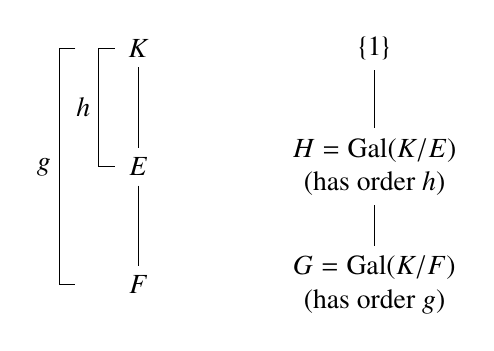
\begin{tikzpicture}[scale=1, node distance=1.5cm, every text node part/.style={align=center}]
          \node at (0,0) (K) {$K$};
          \node [below of=K] (E) {$E$};
          \node [below of=E] (F) {$F$};
          \draw (K) -- (E) -- (F);
          \draw (-.3, 0) -- (-.5,0) -- (-.5,-1.5) -- (-.3, -1.5);
          \node at (-.7, -.75) () {$h$};
          \draw (-.8, 0) -- (-1,0) -- (-1,-3) -- (-.8, -3);
          \node at (-1.2,-1.5) () {$g$};
          \node at (3,0) (1) {$\{1\}$};
          \node [below of=1] (H) {$H = \Gal(K/E)$\\ (has order $h$)};
          \node [below of=H] (G) {$G = \Gal(K/F)$\\ (has order $g$)};
          \draw (1) -- (H) -- (G);
 \end{tikzpicture}
\end{center}
\vspace*{\stretch{1}}
\end{flashcard}

\begin{flashcard}[Fields]{Let $K/F$ be a Galois extension and $G = \Gal(K/F)$. Let $E$ be a subfield of $K$ containing $F$. According to the Fundamental Theorem of Galois Theory, $E/F$ is Galois under what condition? What is the Galois group?}
\vspace*{\stretch{1}}
 $E/F$ is Galois if and only if $\Aut(E/F) \trianglelefteq G = \Gal(K/F)$.\\
 
 $\Gal(E/F) \cong G/H$
 where $H=\text{Gal}(K/E)$
\vspace*{\stretch{1}}
\end{flashcard}

\begin{flashcard}[Fields]{Let $K/F$ be a Galois extension and $G = \Gal(K/F)$. Let $E$ be a subfield of $K$ containing $F$. Let $H = \Gal(K/E)$. According to the Fundamental Theorem of Galois Theory, what can be said about the cosets of $H$ in $G$?}
\vspace*{\stretch{1}}
 There is a one-to-one correspondence between the isomorphisms of $E$ that fix $F$ and the cosets of $H$ in $G$.\\
 
 If $H \trianglelefteq G$, then $\Aut(E/F) = \Gal(E/F) \cong G/H$.
\vspace*{\stretch{1}}
\end{flashcard}

\begin{flashcard}[Fields]{Give an example of a field that is not perfect.}
\vspace*{\stretch{1}}
 Since all fields of characteristic 0 and all finite fields are perfect, we seek an infinite field of characteristic $p$. Recall that a field is perfect if and only if every irreducible polynomial is separable.\\
 
 Consider $\F_p(t)$, the field of rational functions in transcendental $t$. The polynomial $x^p - t \in \F_p(t)[x]$ is irreducible by Eisenstein's using the prime element $t$. Let $\alpha$ be a root. Then $\alpha^p = t$, so $x^p - \alpha^p = (x - \alpha)^p$, which is not separable.
\vspace*{\stretch{1}}
\end{flashcard}

\begin{flashcard}[Fields]{What is the degree of the extension $\F_{p^n}/\F_p$?}
\vspace*{\stretch{1}}
 $[\F_{p_n}:\F_p] = n$
\vspace*{\stretch{1}}
\end{flashcard}

\begin{flashcard}[Fields]{True or False: The field $\F_{p^n}$ is always Galois over $\F_p$. Give a proof or counterexample.}
\vspace*{\stretch{1}}
 True. \\
 
 $\F_{p^n}$ is the splitting field of the separable polynomial $x^{p^n} - x$ and hence it is a Galois extension.
\vspace*{\stretch{1}}
\end{flashcard}

\begin{flashcard}[Fields]{What is the Galois group of $\F_{p^n}/\F_p$?}
\vspace*{\stretch{1}}
 It is the cyclic group of order $n$ generated by the Frobenius automorphism, i.e.\\
 
 $\Gal(\F_{p^n}/\F_p) = \langle \sigma_p \rangle \cong \Z/n\Z$\\
 
 where $\sigma_p: \F_{p^n} \to \F_{p^n}$ so that $\sigma_p(\alpha) = \alpha^p$.
\vspace*{\stretch{1}}
\end{flashcard}

\begin{flashcard}[Fields]{Under what condition on $n,m$ is is true that $\F_{p^n} \subseteq \F_{p^m}$?}
\vspace*{\stretch{1}}
 This is true only when $n$ divides $m$.
\vspace*{\stretch{1}}
\end{flashcard}

\begin{flashcard}[Fields]{Prove that the irreducible polynomial $x^4 + 1 \in \Z[x]$ is reducible modulo every prime.}
\vspace*{\stretch{1}}
 If $p=2$, then $x^4+1 = (x+1)^4$ and so it is reducible.\\
 
 If $p$ is odd, note that $p^2-1$ is divisible by 8. Thus $x^{p^2 - 1} - 1$ is divisible by $x^8-1$. Then
 $$
 x^4+1 \divides x^8 - 1 \divides x^{p^2 - 1} - 1 \divides x^{p^2}-x,
 $$
 the last of which generates $\F_{p^2}$, an extension of degree 2. So any extension generated by a root of $x^4 +1$ is of degree at most 2, which means it is not irreducible over $\F_p$.
\vspace*{\stretch{1}}
\end{flashcard}

\begin{flashcard}[Fields]{Let $p(x)$ be irreducible over $\F_{p^n}$ and let $\alpha$ be a root of $p(x)$. What can we say about the field $\F_{p^n}(\alpha)$? Give a proof.}
\vspace*{\stretch{1}}
 $\F_{p^n}(\alpha)$ is the splitting field for $p(x)$\\
 
 Let $\deg(p(x)) = d$. Then $[\F_{p^n}(\alpha):\F_{p^n}] = d$ and since all finite fields of a particular order are isomorphic, $\F_{p^n}(\alpha) \cong \F_{p^{nd}}$. Thus $\alpha$ is a root of $x^{p^{nd}} - x$. Since $x^{p^{nd}} - x$ contains precisely all irreducible polynomials of degree dividing $nd$, we know $p(x) \divides x^{p^{nd}} - x$ and so all roots of $p(x)$ are in $\F_{p^n}(\alpha)$.
\vspace*{\stretch{1}}
\end{flashcard}

\begin{flashcard}[Fields]{Describe one method for recursively producing irreducible polynomials over $\F_p$.}
\vspace*{\stretch{1}}
 $x^{p^n} - x$ is precisely the product of all irreducible polynomials over $\F_p$ of degree $d$ dividing $n$. \\
 
 For example, say we seek all irreducible degree 6 polynomials over $\F_3$. Since $1,2,3,6$ are the divisors of 6, take $x^{3^6} - x$ and divide by all irreducible polynomials of degrees 1, 2, and 3. The divisors of the quotient are all the irreducible degree 6 polynomials.
\vspace*{\stretch{1}}
\end{flashcard}

\begin{flashcard}[Fields]{Prove that $x^{p^n} - x$ is the product of all irreducible polynomials over $\F_p$ with degree $d$ dividing $n$.}
\vspace*{\stretch{1}}
 The roots of $\F_{p^n}$ are precisely the roots of $x^{p^n} - x$. We know that $\F_{p^d} \subseteq \F_{p^n}$ if and only if $d \divides n$. Extending $\F_p$ to the splitting field of any degree $d$ irreducible polynomial will result in $\F_{p^d}$ since all finite fields of the same size are isomorphic. Thus every minimal polynomial of degree $d$ splits in $\F_{p^d}$. Grouping together all minimal polynomials of the same degree, we see that their product is $x^{p^n} - x$.
\vspace*{\stretch{1}}
\end{flashcard}

\begin{flashcard}[Fields]{What is the \underline{algebraic closure of $\F_p$}?}
\vspace*{\stretch{1}}
 $$
 \overline{\F_p} = \bigcup_{n \geq 1} \F_{p^n}
 $$
\vspace*{\stretch{1}}
\end{flashcard}

\begin{flashcard}[Fields]{Suppose $K/F$ is Galois and $F'/F$ is any extension. Prove that $KF'/F'$ is also Galois. What is its Galois group?}
\vspace*{\stretch{1}}
 $K/F$ is Galois, so $\exists$ separable $p(x)$ such that $K$ is its splitting field. This same polynomial is separable over $F'$, so its splitting field over $F'$ is $KF'$. Thus $KF'/F'$ is Galois. 
\begin{center}
     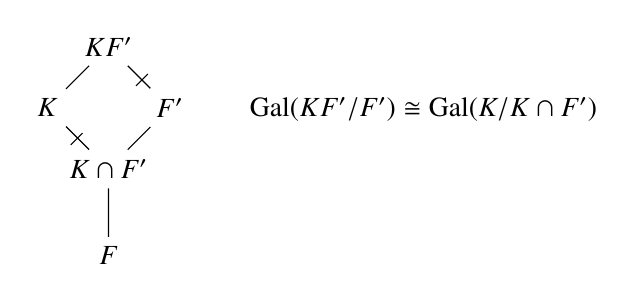
\begin{tikzpicture}[scale=1, node distance=1.1cm]
           \node (KF') {$KF'$};
           \node [below left of=KF'] (K) {$K$};
           \node [below right of=KF'] (F') {$F'$};
           \node [below left of=F'] (KcapF') {$K \cap F'$};
           \node [below of=KcapF'] (F) {$F$};
           \draw (KcapF') -- (K) -- (KF') -- (F') -- (KcapF') --(F);
           \draw (.35,-.5) -- (.50,-.35);
           \draw (-.48,-1.25) -- (-.33,-1.10);
           \node at (4,-.8) {$\Gal(KF'/F') \cong \Gal(K/K \cap F')$};
      \end{tikzpicture}
\end{center}
\vspace*{\stretch{1}}
\end{flashcard}

\begin{flashcard}[Fields]{Complete the formula: Suppose $K/F$ is Galois and $F'/F$ is any extension. \\Then $[KF':F] = $ \blank.}
\vspace*{\stretch{1}}
 $$
 [KF':F] = \dfrac{[K:F][F':F]}{[K \cap F' : F]}
 $$
\vspace*{\stretch{1}}
\end{flashcard}

\begin{flashcard}[Fields]{Let $K_1, K_2$ be Galois extensions of a field $F$. Prove that $K_1 \cap K_2$ is Galois over $F$.}
\vspace*{\stretch{1}}
 Recall that an extension is Galois if and only any irreducible polynomial that has at least one root in the extension splits completely in the extension.\\
 
 Let $p(x)$ be irreducible in $F[x]$ with a root $\alpha$ in $K_1 \cap  K_2$. By the above characterization of Galois extensions, all roots of $p(x)$ are in both $K_1$ and $K_2$. But then all roots of $p(x)$ are in $K_1 \cap K_2$ and so $K_1 \cap K_2$ is Galois.
\vspace*{\stretch{1}}
\end{flashcard}

\begin{flashcard}[Fields]{Let $K_1,K_2$ be Galois extensions of $F$. Is $K_1K_2$ Galois? If so, what is its Galois group?}
\vspace*{\stretch{1}}
 Yes, $K_1K_2$ is Galois. \\
 
 Its Galois group is isomorphic to the subgroup
 $$
 H = \{(\sigma, \tau) \mid \sigma \mid_{K_1 \cap K_2} = \tau \mid_{K_1 \cap K_2}\}
 $$
 of the direct product $\Gal(K_1/F) \times \Gal(K_2/F)$ consisting of elements whose restrictions to the intersection $K_1 \cap K_2$ are equal.
\vspace*{\stretch{1}}
\end{flashcard}

\begin{flashcard}[Fields]{What is the \underline{Galois closure} of finite \\separable extension $E/F$?}
\vspace*{\stretch{1}}
 The \emph{Galois closure} is an extension $K/F$ which is Galois over $F$ and is minimal in the sense that in a fixed algebraic closure of $K$, any other Galois extension of $F$ containing $E$ contains $K$.\\
 
 Note that the Galois closure is defined for \emph{finite separable} extensions.
\vspace*{\stretch{1}}
\end{flashcard}

\begin{flashcard}[Fields]{Prove that if $K/F$ is finite and separable, then $K/F$ is simple.}
\vspace*{\stretch{1}}
 Let $L$ be the Galois closure of $K/F$. By the Fundamental Theorem of Galois Theory, any intermediate field between $K$ and $F$ corresponds to a subgroup of $\Gal(L/F)$. Since there are finitely many subgroups, there are also finitely many intermediate fields. By Artin's Theorem, $K/F$ is simple.
\vspace*{\stretch{1}}
\end{flashcard}

\begin{flashcard}[Fields]{What is a \underline{separable} field extension?}
\vspace*{\stretch{1}}
 A field extension is \emph{separable} if the minimal polynomial of every element is separable.
\vspace*{\stretch{1}}
\end{flashcard}

\begin{flashcard}[Fields]{Prove that any finite field extension over a field of characteristic 0 is simple.}
\vspace*{\stretch{1}}
 Any finite extension $K/F$ of a field of characteristic 0 is separable. If the extension is finite and separable, we can consider its Galois closure. The corresponding Galois group of this Galois closure has finitely many subgroups and thus $K/F$ has only finitely many intermediate fields. By Artin's Theorem, $K/F$ is simple.
\vspace*{\stretch{1}}
\end{flashcard}

\begin{flashcard}[Fields]{Let $\Q(\zeta_n)$ be the cyclotomic field of $n^{th}$ roots of unity. What is its Galois group?}
\vspace*{\stretch{1}}
 Its Galois group is the multiplicative group $(\Z/n\Z)^\times$.
\vspace*{\stretch{1}}
\end{flashcard}

\begin{flashcard}[Fields]{Let $\Q(\zeta_p)$ be the cyclotomic field extension over $\Q$ for prime $p$. What is the Galois group of this extension?}
\vspace*{\stretch{1}}
 The cyclic group $\Z/(p-1)\Z$. 
\vspace*{\stretch{1}}
\end{flashcard}

\begin{flashcard}[Fields]{Let $n = p_1^{\alpha_1} p_2^{\alpha_2} \cdots p_k^{\alpha_k}$ be the factorization of positive integer $n$ into distinct prime powers. Prove that $\Gal(\Q(\zeta_n)/\Q) \cong \Gal(\Q(\zeta_{p_1^{\alpha_1}})/\Q) \times \cdots \times \Gal(\Q(\zeta_{p_k^{\alpha_k}})/\Q).$}
\vspace*{\stretch{1}}
 Note that $\zeta_n^{p_2^{\alpha_2} \cdots p_k^{\alpha_k}}$ is a primitive $p_1^{\alpha_1}$-th root of unity, so the field $\Q(\zeta_{p_1^{\alpha_1}})$ is a subfield of $\Q(\zeta_n)$. The same applies to the other prime powers. Their composite field is $\Q(\zeta_n)$ and their intersection is $\Q$. This means that the Galois group of $\Q(\zeta_n)$ is the direct product of the Galois groups of each of the aforementioned subfields, i.e.
 $$
 \Gal(\Q(\zeta_n)/\Q) \cong \Gal(\Q(\zeta_{p_1^{\alpha_1}})/\Q) \times \cdots \times \Gal(\Q(\zeta_{p_k^{\alpha_k}})/\Q)
 $$
\vspace*{\stretch{1}}
\end{flashcard}

\begin{flashcard}[Fields]{What is an \underline{abelian} field extension?}
\vspace*{\stretch{1}}
 The extension $K/F$ is called \emph{abelian} if $K/F$ is Galois and $\Gal(K/F)$ is an abelian group.
\vspace*{\stretch{1}}
\end{flashcard}

\begin{flashcard}[Fields]{Let $G$ be a finite abelian group. Prove that there is a field $K/\Q$ such that $\Gal(K/\Q) \cong G$.}
\vspace*{\stretch{1}}
 The FTFGAG guarantees that $G \cong \Z_{n_1} \times \cdots \times \Z_{n_k}$. Let $p_i$ be prime such that $p_i \cong 1 \mod n_i$ (there are infinitely many such primes) for $i = 1, \ldots, k$. Let $n = p_1 \cdots p_k$. Then $(\Z/n\Z)^\times \cong  \prod_{i=1}^k (\Z/p_i\Z)^\times \cong  \prod_{i=1}^k \Z/(p_i - 1)\Z$. Since $n_i \divides (p_1 - 1)$, there exists $H_i \leq \Z/(p_i-1)\Z$ such that the quotient by $H_i$ is cyclic of order $n_i$. \\
 
 
 By the fundamental theorem of Galois theory, there is a subfield of $\Q(\zeta_n)$ that is Galois over $\Q$ and has $G$ as its Galois group.
\vspace*{\stretch{1}}
\end{flashcard}

\begin{flashcard}[Fields]{What is the \underline{discriminant} of a polynomial?}
\vspace*{\stretch{1}}
 Let $x_1, \ldots, x_n$ be the roots of a polynomial. Then the discriminant of the polynomial is $D = \displaystyle \prod_{i<j}(x_i - x_j)^2$
\vspace*{\stretch{1}}
\end{flashcard}

\begin{flashcard}[Fields]{What can we say about the Galois group of a polynomial if the square root of its discriminant is an element of the base field?}
\vspace*{\stretch{1}}
 The Galois group contains automorphisms that fix the base field, so if $\sqrt{D} = \displaystyle \prod_{i<j} (x_i - x_j)$ is contained in the base field, the any automorphism in the Galois gorup fixes $\sqrt{D}$. This means that the number of transpositions of the roots is even, since an odd number of transpositions would change the sign of $\sqrt{D}$. We conclude that the Galois group is a subgroup of $A_n$ where $n$ is the degree of the polynomial in question.
\vspace*{\stretch{1}}
\end{flashcard}

\begin{flashcard}[Fields]{Discuss the Galois group of a general irreducible cubic polynomial.}
\vspace*{\stretch{1}}
 The Galois group must be a subgroup of $S_3$ and have order at least 3 since adjoining a single root will already result in an extension of degree 3. If the discriminant is a square of an element of the base field, then the Galois group in $A_3$, i.e. it's precisely $A_3$. If the discriminant is not a square, then the Galois group must properly contain $A_3$, i.e. it's precisely $S_3$.
\vspace*{\stretch{1}}
\end{flashcard}

\begin{flashcard}[Fields]{List the transitive subgroups of $S_4$. What is the significance of this list of subgroups of $S_4$ for Galois theory?}
\vspace*{\stretch{1}}
 The transitive subgroups of $S_4$ are $S_4$, $A_4$, $D_8$, $V_4$, and $\Z/4\Z$.\\
 
 These are the only possible Galois groups for an irreducible degree 4 polynomial.
\vspace*{\stretch{1}}
\end{flashcard}

\begin{flashcard}[Fields]{List the transitive subgroups of $S_5$. What is the significance of this list of subgroup of $S_5$ for Galois theory?}
\vspace*{\stretch{1}}
 The transitive subgroups of $S_5$ are $S_5$, $A_5$, $D_{10}$, $F_{20}$, and $\Z/5\Z.$
 
 These are the only possible Galois groups for an irreducible degree 5 polynomial.
\vspace*{\stretch{1}}
\end{flashcard}

\begin{flashcard}[Fields]{What is a \underline{cyclic} extension?}
\vspace*{\stretch{1}}
 An extension $K/F$ is \emph{cyclic} if it is Galois with a cyclic Galois group.
\vspace*{\stretch{1}}
\end{flashcard}

\begin{flashcard}[Fields]{Let $F$ be a field of characteristic not dividing $n$. Let $F$ contain the $n^{th}$ roots of unity. Prove that $F(\sqrt[n]{a})$ for $a \in F$ is Galois over $F$.}
\vspace*{\stretch{1}}
 The minimal polynomial for $\sqrt[n]{a}$ is $x^n - a$. This polynomial is separable. Since adjoining $\sqrt[n]{a}$ generates the splitting field, the extension is Galois.
\vspace*{\stretch{1}}
\end{flashcard}

\begin{flashcard}[Fields]{What does it mean if an element $\alpha$ that is algebraic over $F$ can be \underline{expressed by radicals}?}
\vspace*{\stretch{1}}
 An element $\alpha$ can be \emph{expressed by radicals} if $\alpha$ is an element of a field $K$ that can be formed by a succession of simple radical extensions
 $$F = K_0 \subset K_1 \subset \cdots \subset K_s = K$$
 where $K_{i+1} = K_i(\sqrt[n_i]{a_i})$ for some $a_i \in K_i$.
\vspace*{\stretch{1}}
\end{flashcard}

\begin{flashcard}[Fields]{What does it mean for a polynomial $f(x) \in F[x]$ to be \underline{solvable by radicals}?}
\vspace*{\stretch{1}}
 A polynomial is \emph{solvable by radicals} if all its roots can be expressed by radicals.
\vspace*{\stretch{1}}
\end{flashcard}

\begin{flashcard}[Fields]{Complete the sentence: A polynomial $f(x)$ can be solved by radicals if and only if \blank .}
\vspace*{\stretch{1}}
 its Galois group is a solvable group
\vspace*{\stretch{1}}
\end{flashcard}

\begin{flashcard}[Fields]{True or False: No quintic polynomial is solvable by radicals. Give a proof or counterexample.}
\vspace*{\stretch{1}}
 False. \\
 
 This is true if and only if the Galois group of the polynomial is $S_5$ or $A_5$, which are both not solvable groups. For example, $f(x) = x^5 - 6x+3 \in /Q[x]$ has Galois group $S_5$ and so it is not solvable by radicals. But $g(x) = x^5 - 1$ contains the $5^{th}$ roots of unity, so this polynomial is solvable by radicals.
\vspace*{\stretch{1}}
\end{flashcard}

\begin{flashcard}[Fields]{Let $p$ be a prime not dividing the discriminant $D$ of $f(x) \in \Z[x]$. What relationship does the Galois group of over $\Q$ of $f(x)$ have to the Galois group over $\F_p$ of $\overline{f(x)}$?}
\vspace*{\stretch{1}}
 The Galois group of $\overline{f(x)}$ is isomorphic to a subgroup of the Galois group of $f(x)$.
\vspace*{\stretch{1}}
\end{flashcard}

% \begin{flashcard}[Fields]{front}
% \vspace*{\stretch{1}}
%  back
% \vspace*{\stretch{1}}
% \end{flashcard}
% 
% \begin{flashcard}[Fields]{front}
% \vspace*{\stretch{1}}
%  back
% \vspace*{\stretch{1}}
% \end{flashcard}
% 
% \begin{flashcard}[Fields]{front}
% \vspace*{\stretch{1}}
%  back
% \vspace*{\stretch{1}}
% \end{flashcard}
% 
% \begin{flashcard}[Fields]{front}
% \vspace*{\stretch{1}}
%  back
% \vspace*{\stretch{1}}
% \end{flashcard}
% 
% \begin{flashcard}[Fields]{front}
% \vspace*{\stretch{1}}
%  back
% \vspace*{\stretch{1}}
% \end{flashcard}
% 
% \begin{flashcard}[Fields]{front}
% \vspace*{\stretch{1}}
%  back
% \vspace*{\stretch{1}}
% \end{flashcard}
% 
% \begin{flashcard}[Fields]{front}
% \vspace*{\stretch{1}}
%  back
% \vspace*{\stretch{1}}
% \end{flashcard}





















\begin{flashcard}[Fields]{Complete the sentence: An algebraic extension over a field of characteristic 0 is \blank.}
\vspace*{\stretch{1}}
 separable
\vspace*{\stretch{1}}
\end{flashcard}

\begin{flashcard}[Fields]{What is the Frobenius map? What is its relation to the Galois group of a finite extension over a finite field?}
\vspace*{\stretch{1}}
 In a field of characteristic $p$, the Frobenius map is the map $\sigma: a \to a^p$ for any element $a$ in the field. \\
 
 A finite extension of a finite field is cyclic, and the Galois group is generated by the Frobenius map.
\vspace*{\stretch{1}}
\end{flashcard}








\begin{flashcard}[Miscellaneous]{State Zorn's lemma.}
\vspace*{\stretch{1}}
 Suppose a partially ordered set P has the property that every chain (i.e. totally ordered subset) has an upper bound in P. Then the set P contains at least one maximal element.
\vspace*{\stretch{1}}
\end{flashcard}

\begin{flashcard}[Miscellaneous]{What is an \underline{equivalence relation}?}
\vspace*{\stretch{1}}
 An equivalence relation is a binary relation on a set that is reflexive, symmetric, and transitive.
\vspace*{\stretch{1}}
\end{flashcard}

\end{document}



% 
% 
% 
% 
% \begin{flashcard}[topic]{front}
% \vspace*{\stretch{1}}
%  back
% \vspace*{\stretch{1}}
% \end{flashcard}


